
\section{平面的なグラフの性質}

グラフの平面性を特徴付ける性質は1930年に
ロシアの数学者クラトフスキーが初めて正確に記述した。
その後約半世紀を経て平面性を判定する線形時間アルゴリズムが提案され、
言語実装に至ったのは90年代。
現在は様々な定理・補題を礎に100行程度で記述できるまで簡潔になっている。
ここでは代表的な三つの定理を通して平面的グラフの基本的な性質を確認する。



\subsection{オイラーの多面体公式}
オイラーの多面体公式は、
グラフが非平面的であることの緩い必要条件を記述する側面を持つ。
辺の個数が$3n-6$より多ければ非平面的と判定できる。
ただし$3n-6$以下のグラフであっても非平面的なグラフは存在するため、
緩い必要条件でグラフを平面的と決めつける判定方法は偽陽性を持つ。


\begin{theorem}[オイラーの多面体公式]
連結な平面的グラフ$G$が$n$個の頂点、$m$個の辺、そして
$f$個の面で構成されているとき、$n - m + f = 2$ が成り立つ。
\end{theorem}
\vspace*{-0.7\intextsep}
\setcolumnwidth{0.666\textwidth, 0.333\textwidth}
\begin{paracol}{2}
\begin{proof}
$G$ が辺を持たない自明なグラフなら%$n=f=1,~m=0$で
$1+0+1=2$。
辺の個数が$m-1$の任意の連結な平面的グラフで主張が成り立つと仮定する。
$G$の任意の辺$e$に関して次の二つの重複する場合分けを考える。

$e$が自己ループでも多重辺でもないなら$e$の縮約$G / e$は
$n-1$個の頂点と$m-1$個の辺、$f$個の面を持つ。
ただし、この辺縮約は副次的に生成される多重辺を削除しないものとする。
また、$e$ が橋でないなら$e$を削除して得られるグラフ$G \setminus e$は
$n$個の頂点、$m-1$個の辺、そして$f-1$個の面を持つ。
いずれも帰納法の仮定から$n - m + f = 2$を得る。
\end{proof}

\switchcolumn
%\vspace{.5\intextsep}
\centering
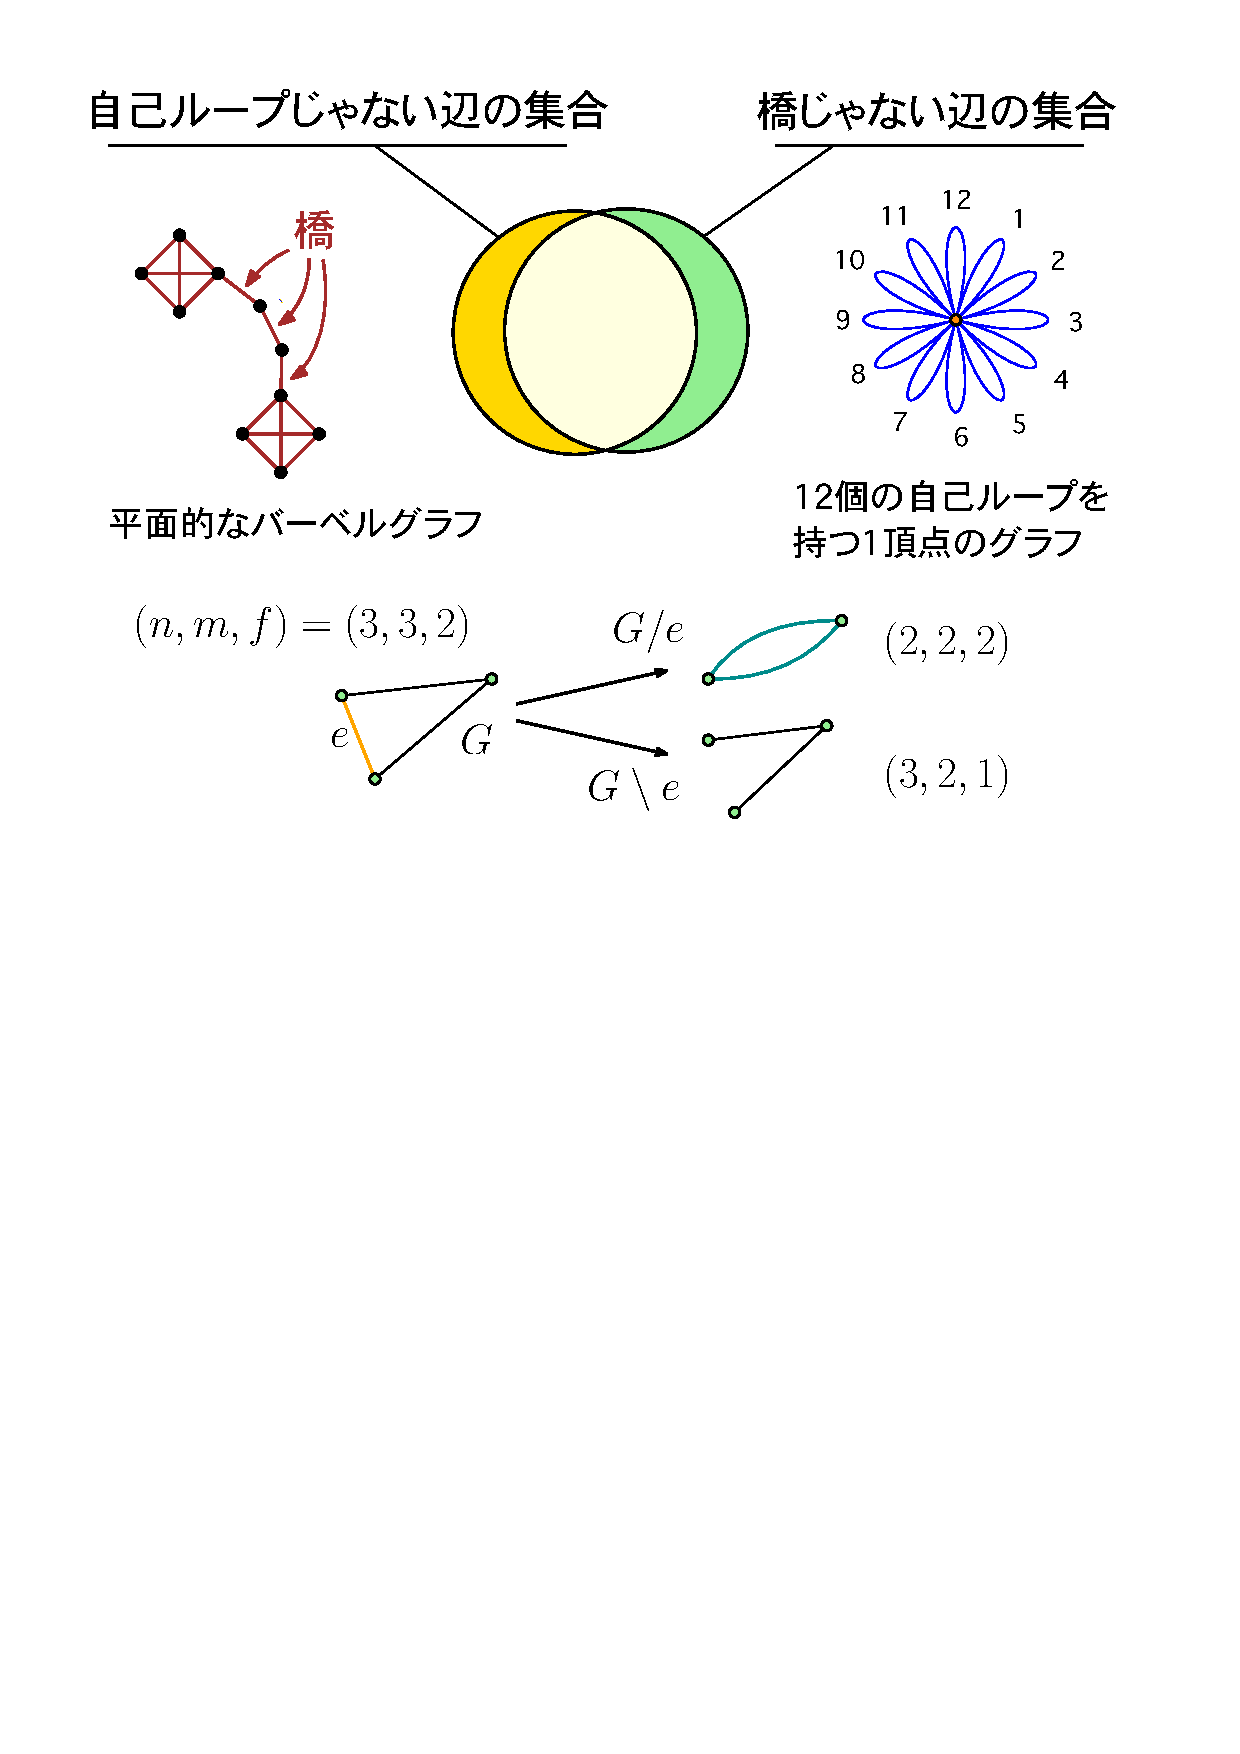
\includegraphics[width=0.32\textwidth]{figures/sample_figure_in_proof_of_eular_formula.pdf}
\end{paracol}



\begin{corollary}
\label{coro:girth}
単純で連結な平面的グラフ$G=(V, E)$が$|V|\geq 3$で、
内周が定数$\gamma$で抑えられるなら
$|E| \leq \frac{\gamma}{\gamma - 2}(|V| - 2)$が成り立つ。
\end{corollary}

\begin{proof}
握手補題からの類推より$\gamma |F| \leq 2|E|$を得る。
オイラーの多面体公式より$|V|-|E|+\frac{2}{\gamma}|E| \geq 2$。
この式を整理すると主張を得る。
\end{proof}

\begin{lemma}[握手補題]
グラフ$G=(V, E)$の次数の合計は辺の個数の$2$倍、
すなわち$\sum\limits_{v \in V}\deg(v)=2|E|$。
\end{lemma}
\vspace*{-0.7\intextsep}
\begin{proof}
各頂点の接続辺数を数え上げると、どの辺も二回カウントされる。
\end{proof}

\begin{corollary}
\label{coro:minimum_nonplanar}
最小頂点数の非平面的グラフは$K_5$。最小辺数の非平面的グラフは$K_{3,3}$。
\end{corollary}


\begin{proof}
$K_5, K_{3,3}$いずれも\cref{coro:girth}より非平面的。
下に連結な単純グラフで$5$頂点以下、
もしくは$6$頂点以上でも$9$辺以下で$2$-連結のグラフを示す。
$K_5$および$K_{3,3}$以外はいずれも平面描画を持つ。
\end{proof}

%\vspace*{.5\intextsep}
%\centering
\noindent
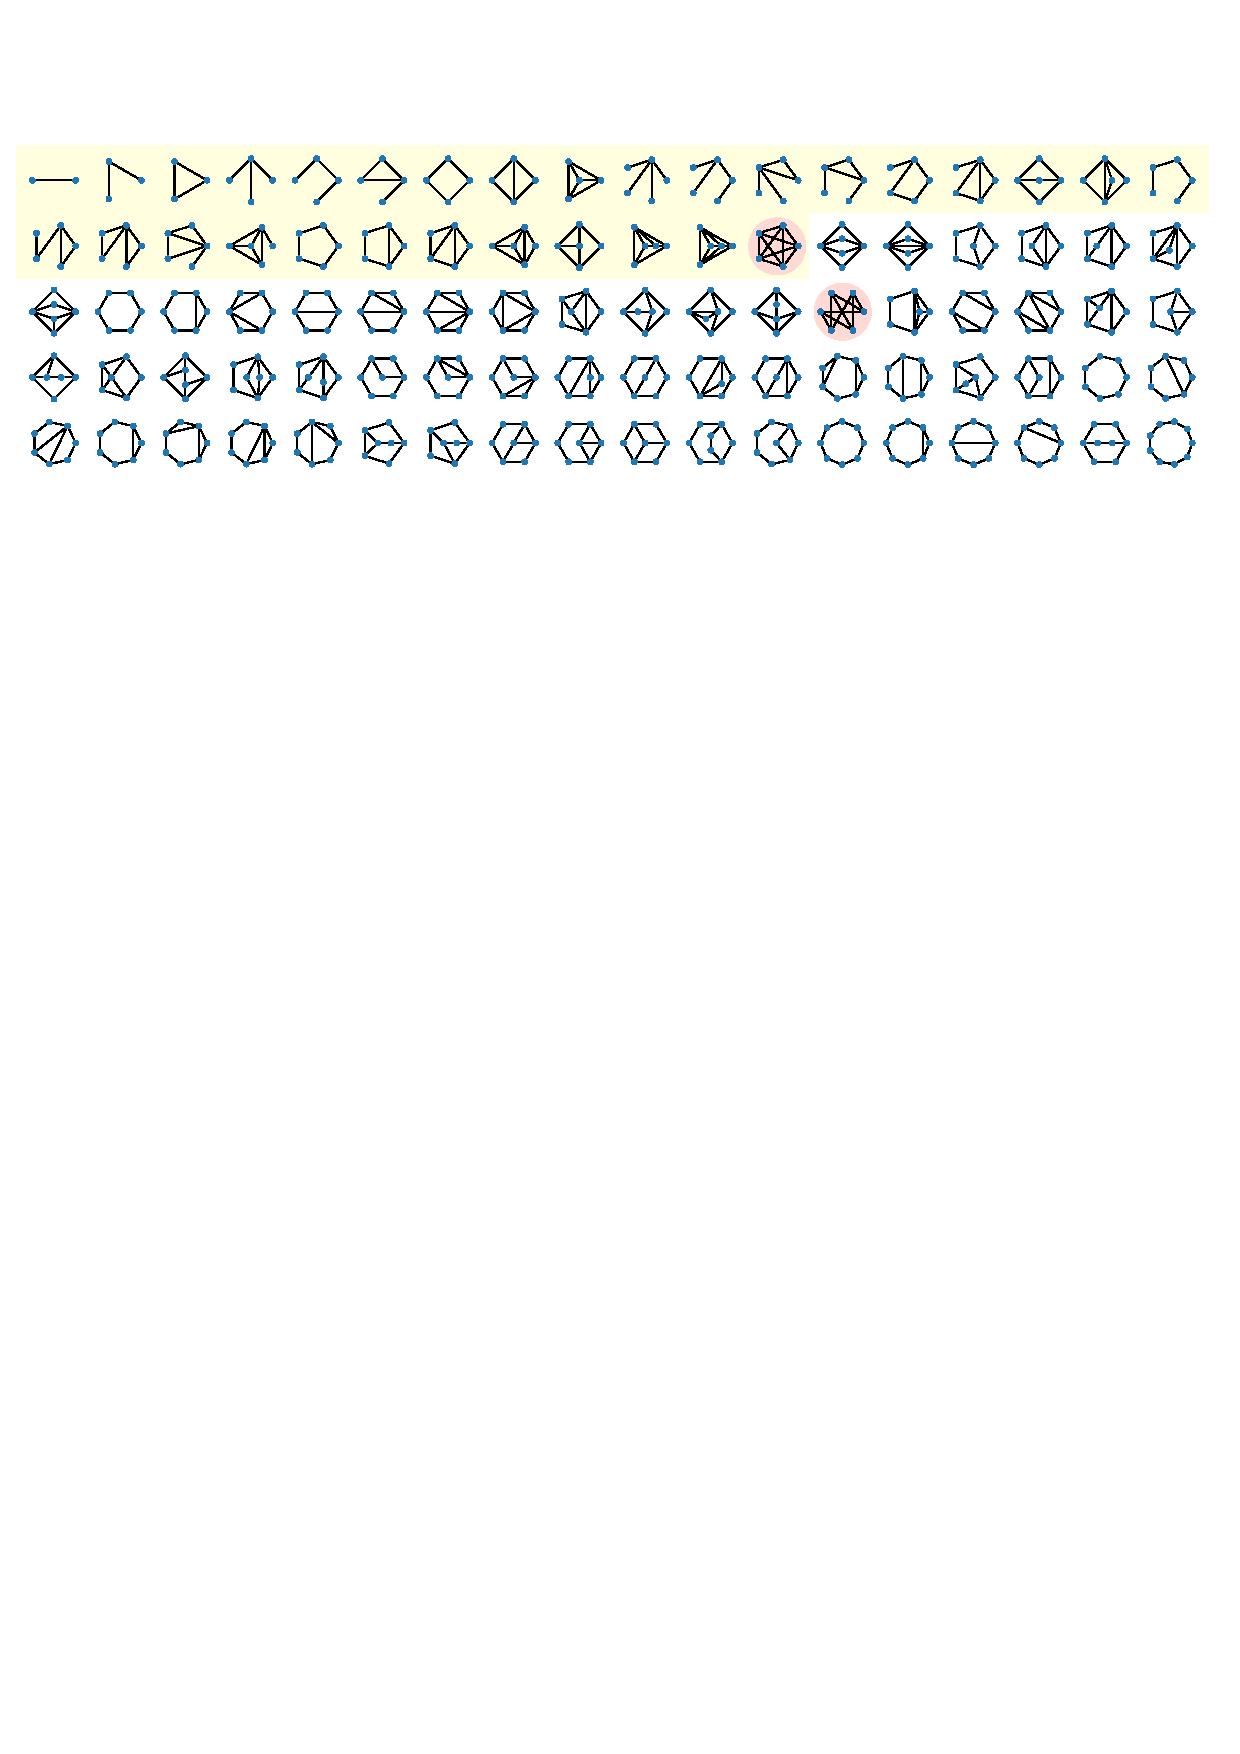
\includegraphics[width=1.0\textwidth]{figures/simple_graphs2.pdf}

\vspace{0.5\intextsep}

$k$-連結性および、極小非平面的グラフは$2$-連結(\cref{lemma:2-connected})は、
それぞれ
第\ref{subsec:tutte}節および第\ref{subsec:kuratowski}節で扱う。
%クラトフスキー\cref{thm:kuratowski}を自明にみえるが、
%本レポートで扱う証明では最小辺数を論拠とする箇所があるため愚直な手続きをとる。



%%%%%%%%%%%%%%%%%%%%%%%%%%%%%%%%%%%%%%%%%%%%%%%%%%%%%%%%%%%%%%%%%%%%%%%%%%%%%%%%%%%%%%%
\subsection{タットの平面描画}\label{subsec:tutte}

ここではタットの平面描画について考察する。
タットの平面描画は1963年にイギリスの数学者タットによって提案された
グラフの描画方法で、平面描画の基礎としての重要な役割を持つ。


\begin{definition}[タットの平面描画]
\label{def:tutte_drawing}
単純で$3$-連結な平面的グラフに対して、
次の三つの制約を満たす描画をタットの平面描画と呼ぶ。
外面境界は凸多角形。
内部の頂点は隣接頂点の重心。各辺は直線分。
\end{definition}


\setcolumnwidth{0.55\textwidth, 0.45\textwidth}
\begin{paracol}{2}
右にタットの平面描画の例を示す。
左は単位正方形内に一様ランダムに生成した
$50$点の集合$S$に対するドロネー三角形分割であり、
右はそれを幾何学的グラフと見做したタットの平面描画である。
定理の第一制約に従い外面境界に$S$の凸包(赤点)をとっている。
このとき第二(隣接重心)・第三(辺直線分)制約を満たすことが確認できる。

\switchcolumn
%\vspace{-1.\intextsep}
\centering
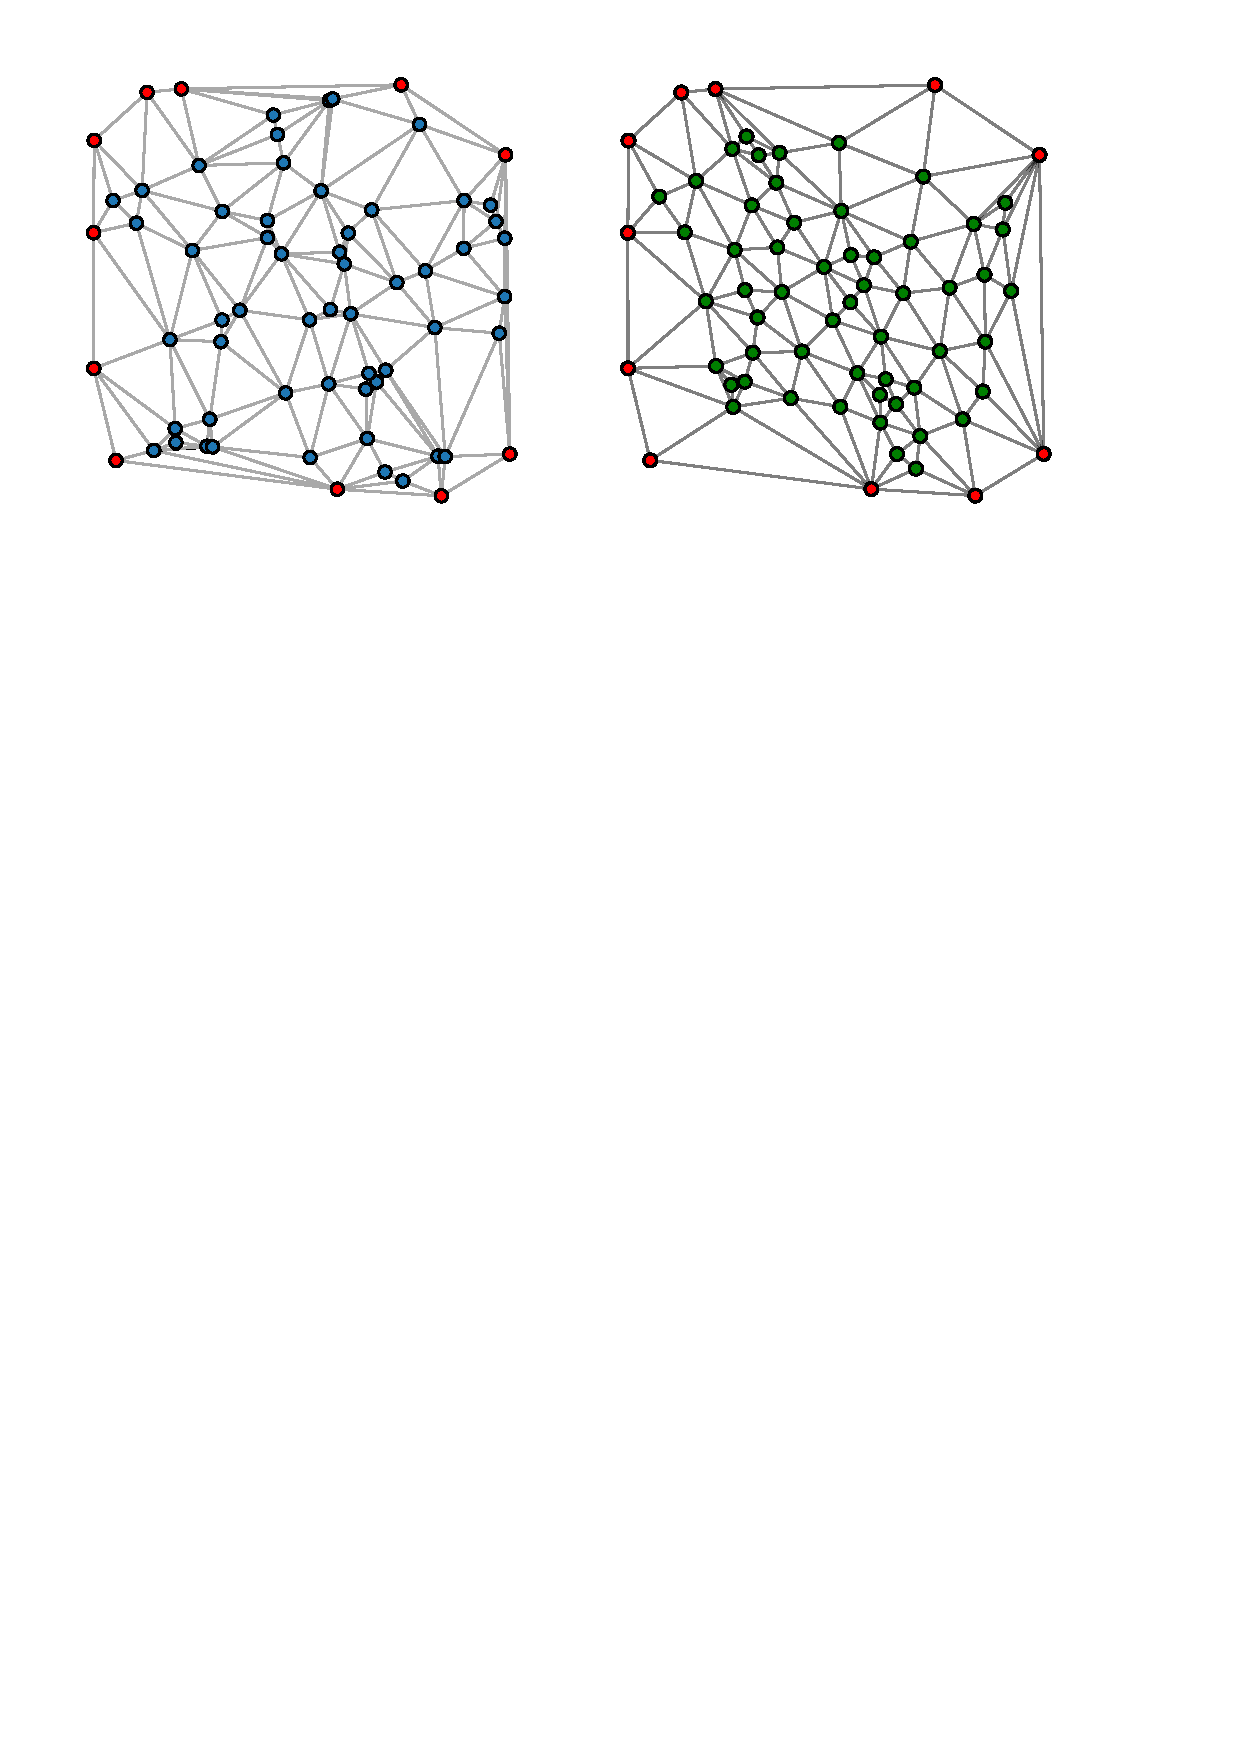
\includegraphics[width=0.4\textwidth]{figures/delaunay_tutte.pdf}
\end{paracol}


\setcolumnwidth{0.85\textwidth, 0.15\textwidth}
\begin{paracol}{2}

\paragraph{$k$-連結性}
\cref{def:tutte_drawing}の前提条件に$3$-連結性が付与されているが、
これは平面描画の縮退を排除するためにある。
連結グラフ$G=(V, E)$の$k$-連結性を任意の整数$k\geq 1$に対して次のように定義する。
どんな$(k-1)$-頂点部分集合$S \subseteq V$を持ってきても
$G \setminus S$が非連結にならないなら$G$は$k$-連結であるという。
また一般的に$k$-連結であれば$(k-1)$-連結である。
右の完全二部グラフ$K_{2,4}$の紫頂点を外面としたタットの平面描画が下段になる。
両端の$2$頂点を削除すると残りは孤立点になるので$K_{2,4}$は$2$-連結グラフである。
このとき外面に属さない頂点は隣接頂点の中点をとるので$2$頂点が一つの座標に収束する。
%これは写像直線分どうしが端点以外の共通部分を持つので平面的ではない。

\switchcolumn
\vspace{1.5\intextsep}
\centering
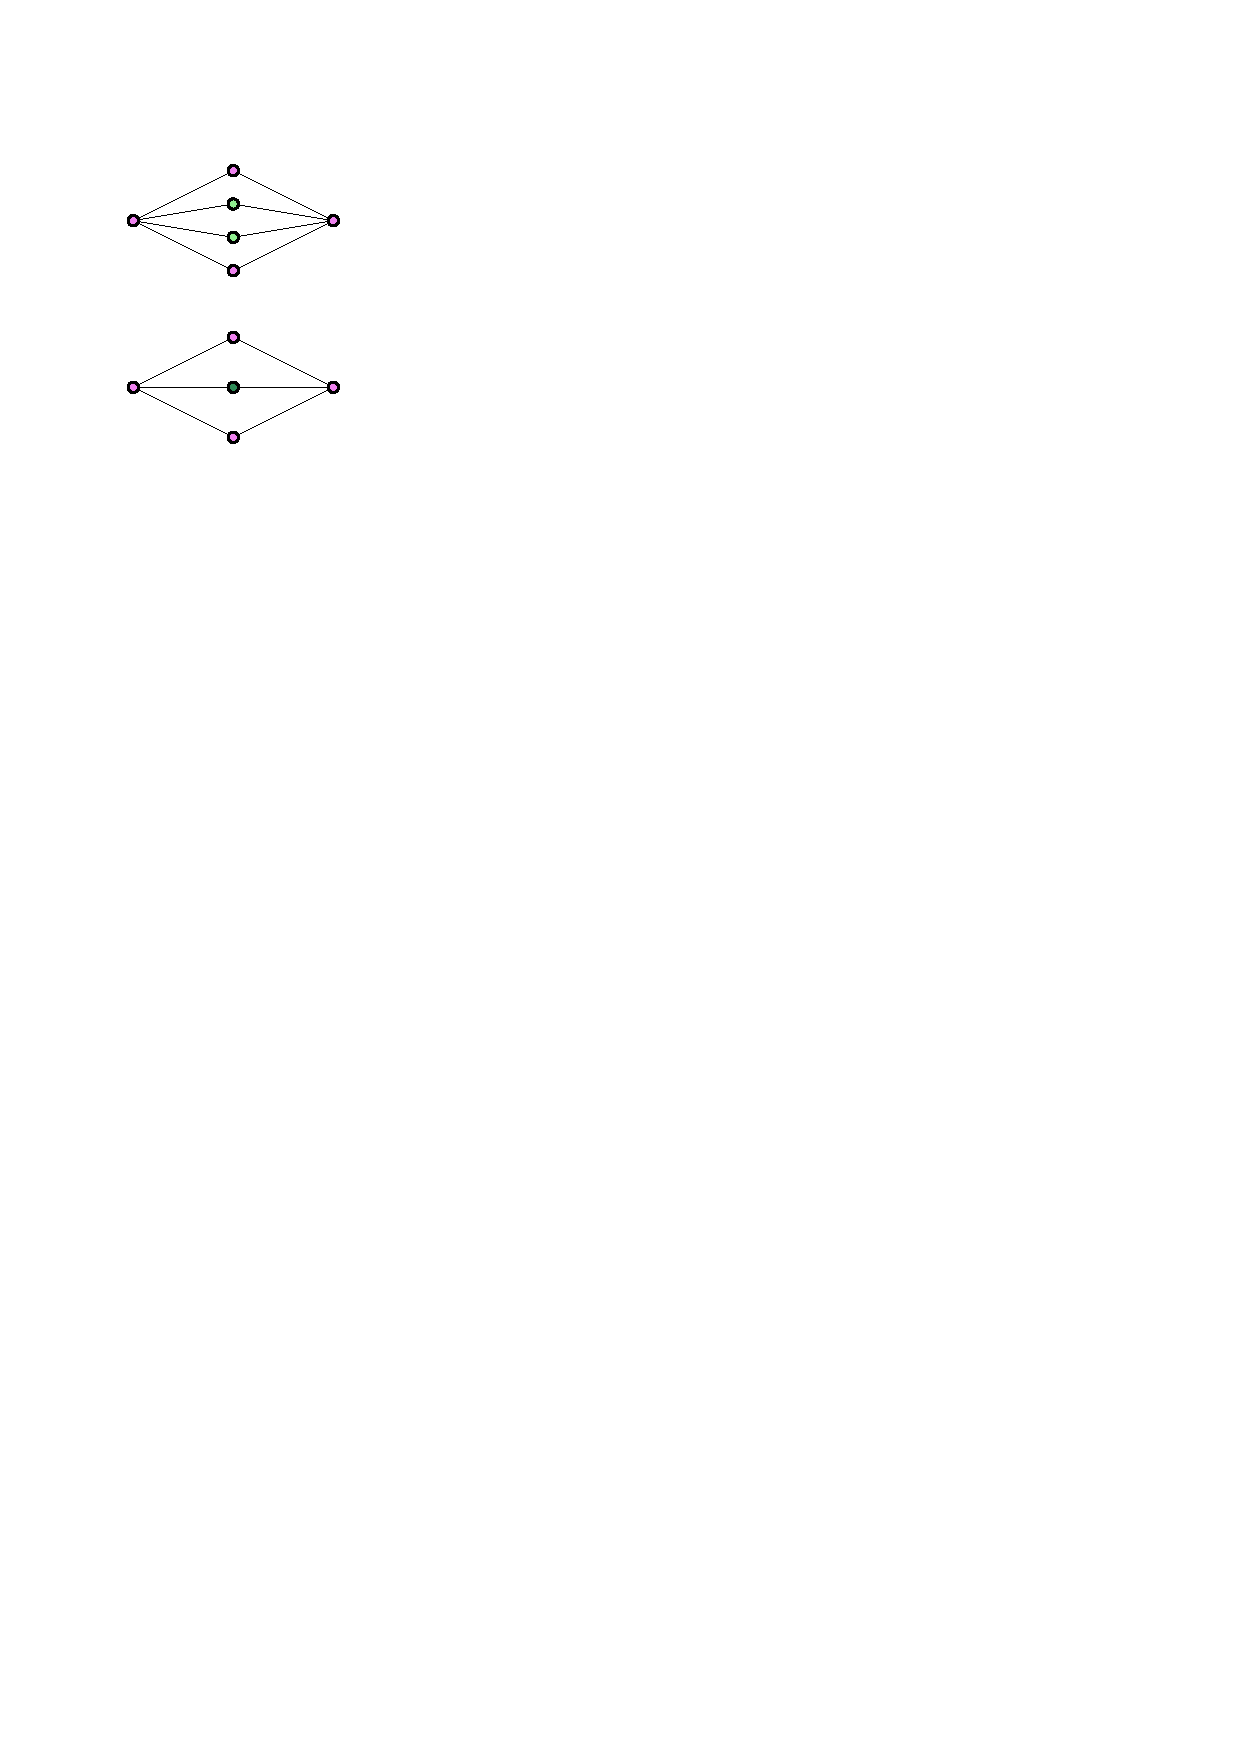
\includegraphics[width=0.12\textwidth]{figures/tutte_degeneracy.pdf}
\end{paracol}


\paragraph{メンガーの定理}
ここで$k$-連結性を特徴付けるメンガーの定理を導入する。
連結性と点素な経路の関係性を記述する非常に使い勝手の良い定理である。
%後述のタットのばね定理およびクラトフスキー定理の証明でも用いている。
二つの$xy$-経路$p_1, p_2$が互いに点素であるとは、
$p_1$と$p_2$の共通頂点が両端点$x,~y$以外に無いことをいう。
%同様に共通する辺を持たない経路対を互いに辺素であるという。
%点素であれば辺素である。

グラフ$G=(V, E)$の頂点集合$A, B \subseteq V$に対して、
頂点集合$S\subseteq V$が$G \setminus S$で$A$から$B$への経路をすべて排除するとき
$S$を$AB$-切断集合という。
$AB$-接続成分を
$A$と$B$を接続し経由頂点が$A \cup B$に属さない経路の集まりから誘導される
$G$の部分グラフとする。
$AB$-接続成分$X$の大きさは$X$に属す$A$と$B$を接続する経路の個数で測られる。

\begin{theorem}[メンガーの定理]
\label{thm:menger}
$G$を連結グラフとし$A, B$を$G$の頂点の部分集合とする。
$G$内のどんな$AB$-切断集合$S$をもってきても$|S| \geq k$なら、
大きさが$k$の$AB$-接続成分$C$が存在する。
\end{theorem}

\setcolumnwidth{0.72\textwidth, 0.28\textwidth}
\begin{paracol}{2}
\begin{proof}
辺の個数に関する構成的な帰納法で示す。
$G$に辺が無いなら$A \cap B$を$C$の頂点集合とすることで主張を満たす。
$G$は$A$から$B$への経路に属す辺$e=(x, y)$を持ち、
$G' = G \setminus e$が大きさ$k$未満の$AB$-切断集合$S$を持つと仮定する。
$P=S\cup\{x\}$および$Q=S\cup\{y\}$はそれぞれ$G$の$AB$-切断集合である。
$|P|=|Q|=|S|+1$。
$G'$の$AP$-切断集合および$QB$-切断集合は、それぞれ
$G$の$AB$-切断集合でもある。
このとき
$G'$は$AP$-接続成分$X$および$QB$-接続成分$Y$を持つ。
$X\cap Y=S$なので$C=(X\cup Y) + e$を得る。
\end{proof}

\switchcolumn
\vspace{0.5\intextsep}
\centering
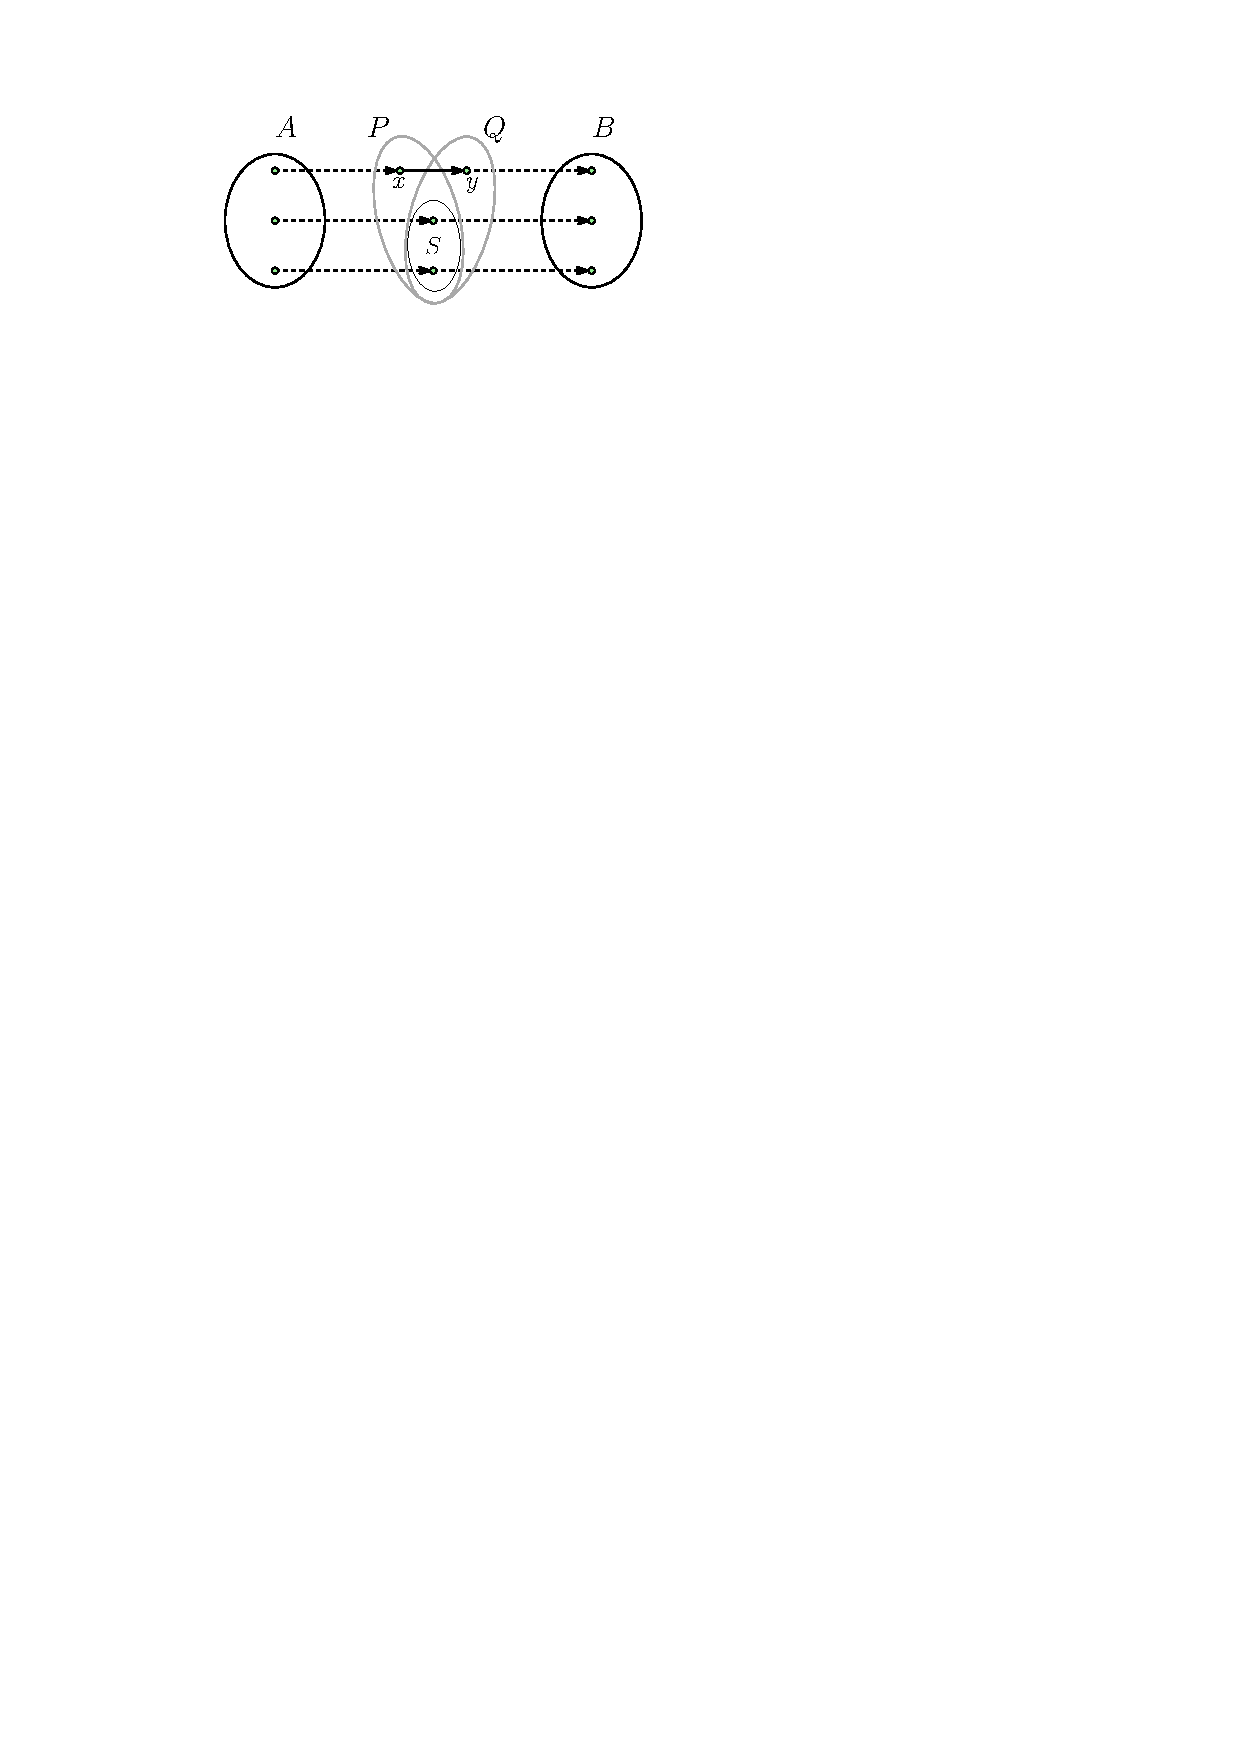
\includegraphics[width=0.27\textwidth]{figures/menger_goring_proof.pdf}
\end{paracol}

$AB$-接続成分$X$に属す$k$個の経路が点素であることは
切断集合に対する$k$の最小性から導ける。
証明の構成からも分かる通り$X$内の経路$p_1, p_2$が共通の経由頂点$v$を持つなら
$v$は$S$に属していなければならず、いずれか一方は冗長であり排除される。
もう少し厳密には以下の系に従う。
$x, y \in V$に対して$S$が次の条件を満たすとき$S$は$x$と$y$を切断するという。
$\{x, y\}\cap S = \varnothing$かつ$x$から$y$へのどんな経路を持ってきても
$S$の頂点を通過する。

\begin{corollary}
\label{coro:pairwise_independent}
$G=(V,E)$を対象グラフとし$s,t\in V$とする。ただし$s \neq t$で$(s, t) \notin E$。
$s$と$t$を切断するどんな集合$S$も$|S|\geq k$なら
非冗長で点素な$st$-経路が$k$個存在する。
\end{corollary}
\begin{proof}
$G'=G\setminus\{s,t\}$および$A=N(s), B=N(t)$とする。
$G'$内のどんな$AB$-切断集合$S$も$G$において$s$と$t$を切断し$|S|\geq k$を満たす。
%そのサイズは少なくとも$k$はある。
メンガーの\cref{thm:menger}より
大きさ$k$の$AB$-接続成分$X$が存在する。
始点として$s$から$A$の各頂点に接続し、
終点として$B$の各頂点から$t$に接続することで$k$個の点素な$st$-経路を得る。
\end{proof}






\paragraph{タットの平面描画の求め方}
$n$-頂点グラフ$G=(V,E)$のタットの平面描画$\Gamma$は、
$xy$-座標それぞれ$n$個の一次式からなる2つの連立方程式を解くことで得られる。
$\Gamma$は任意の$v\in V$に対して
$v$を$\Gamma(v)=(x_v^*, y_v^*) \in \mathbb{R}^2$へ写像する。
外面境界上の頂点集合を$F \subseteq V$とする。
$F$の頂点$v$は凸の位置に固定されるので
一次式$x_v = x_v^*,~ y_v=y_v^*$を得る。
%$F$内の頂点は凸の位置に固定されるので一次式は
%$x_v = x_v^*$および$y_v=y_v^*$となる。
$V \setminus F$内の頂点に関しては
一次式$\deg(v)\cdot x_v - \sum_{w \in N(v)} x_w = 0$および
$\deg(v)\cdot y_v - \sum_{w \in N(v)} y_w = 0$として
隣接頂点の重心に座標値をとる制約として定式化する。


具体的なpythonコードは下記の\lstrefname\ref{lst:tutte}のように書ける。
この例では numpy パッケージを用いる。
\begin{lstlisting}[language=Python, caption=タットの平面描画,label=lst:tutte]
def tutte_embedding(G, F, pos):
    A, Bx, By = [], [], []
    for u in g:
        a, bx, by = [0] * G.number_of_nodes(), 0, 0
        if u in F:
            a[u] = 1
            bx, by = pos[u]
        else:
            a[u] = len(G.neighbors(u))
            for v in G.neighbors(u):
                a[v] = -1
        A.append(a)
        Bx.append(bx)
        By.append(by)
    xcoords = np.linalg.solve(A, Bx)
    ycoords = np.linalg.solve(A, By)
    return {i: (x, y) for i, (x, y) in enumerate(zip(xcoords, ycoords))}
\end{lstlisting}
入力は、対象グラフ{\tt G}と外面境界上の頂点部分集合の{\tt list F}、
{\tt F}内の各頂点の座標情報の{\tt dict pos}。
{\tt G}の頂点は整数識別子で管理されているものとする。
このとき、
連立一次方程式を定義するために係数行列{\tt A}と係数ベクトル{\tt Bx, By}を導入し(第2行)、
制約条件に基づき適宜係数を構成していく(第3-14行)。
そして第15・16行で連立一次方程式ソルバ
{\tt numpy.linalg.solve}を用いて具体的な座標を得る。
最後に頂点から座標値への単射としての連想配列を形成し出力する(第17行)。


\setcolumnwidth{0.75\textwidth, 0.25\textwidth}
\begin{paracol}{2}

\paragraph{包囲閉路}
与えられた$3$-連結な平面的グラフ$G$に対して
正しくタットの平面描画を得るには、
外面境界上の頂点系列を適切に取得する必要がある。
平面埋込みが与えられていれば任意の面を外面として選択%し、
%外面境界上の頂点を自己交差しない凸の位置に配置
すれば適切に平面描画が得られる。
別の言い方をすると、外面境界は包囲閉路であれば平面描画となる。

\switchcolumn
%\vspace{1.5\intextsep}
\centering
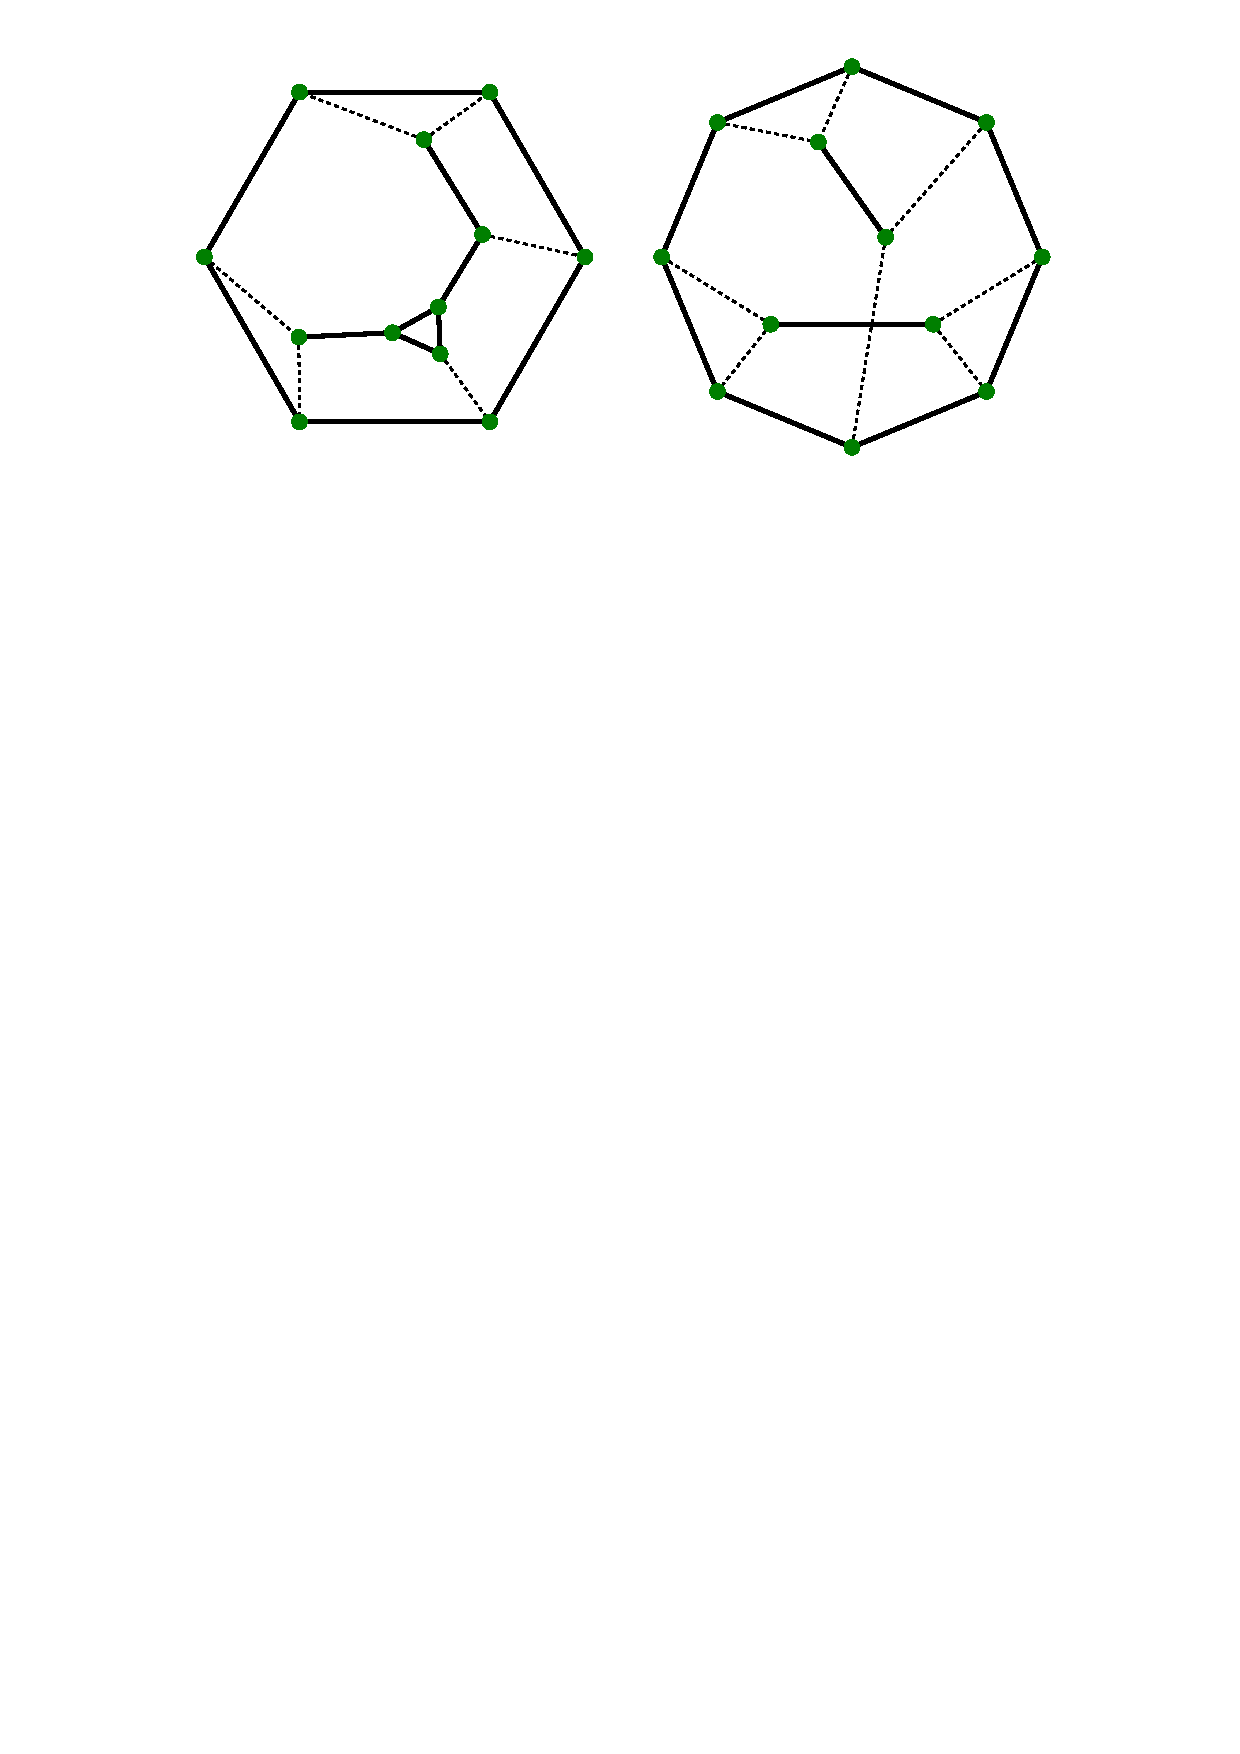
\includegraphics[width=0.24\textwidth]{figures/tutte_frucht_error.pdf}
\end{paracol}
包囲閉路$C$は、
$G\setminus C$が連結で、$C$内で隣接しない頂点間を接続する辺を$E$内に持たない閉路である。
包囲閉路の第二制約は$K_4$の4頂点を外面と選んだ時に対角線どうしが
交差すること排除するための制約である。
右上はフルフトグラフの異なる外面選択時のタットの平面描画を示している。
左は包囲閉路だが右は違う。そのため交差する辺対を持つ。




\paragraph{平面上の右と左}

平面上の$3$点$p_i=(x_i, y_i) \in \mathbb{R}^2,\ i=1, 2, 3$に対して、
向き$\orient(p_1, p_2, p_3)$を次のように行列式を用いて定義する。
\setcolumnwidth{0.85\textwidth, 0.15\textwidth}
\begin{paracol}{2}
\vspace{-1.5\intextsep}
%\[
\begin{align*}
\orient(p_1, p_2, p_3) =
    \left|
        \begin{array}{ccc}
            x_1 & y_1 & 1 \\
            x_2 & y_2 & 1 \\
            x_3 & y_3 & 1
    \end{array}
    \right| &=
    \left|
        \begin{array}{cc}
            x_1 - x_3 & y_1 - y_3 \\
            x_2 - x_3 & y_2 - y_3
        \end{array}
    \right| \\
&=(x_1 - x_3)(y_2 - y_3) - (x_2 - x_3)(y_1 - y_3).
\end{align*}
%\]
\switchcolumn
%\vspace*{1.5\intextsep}
\centering
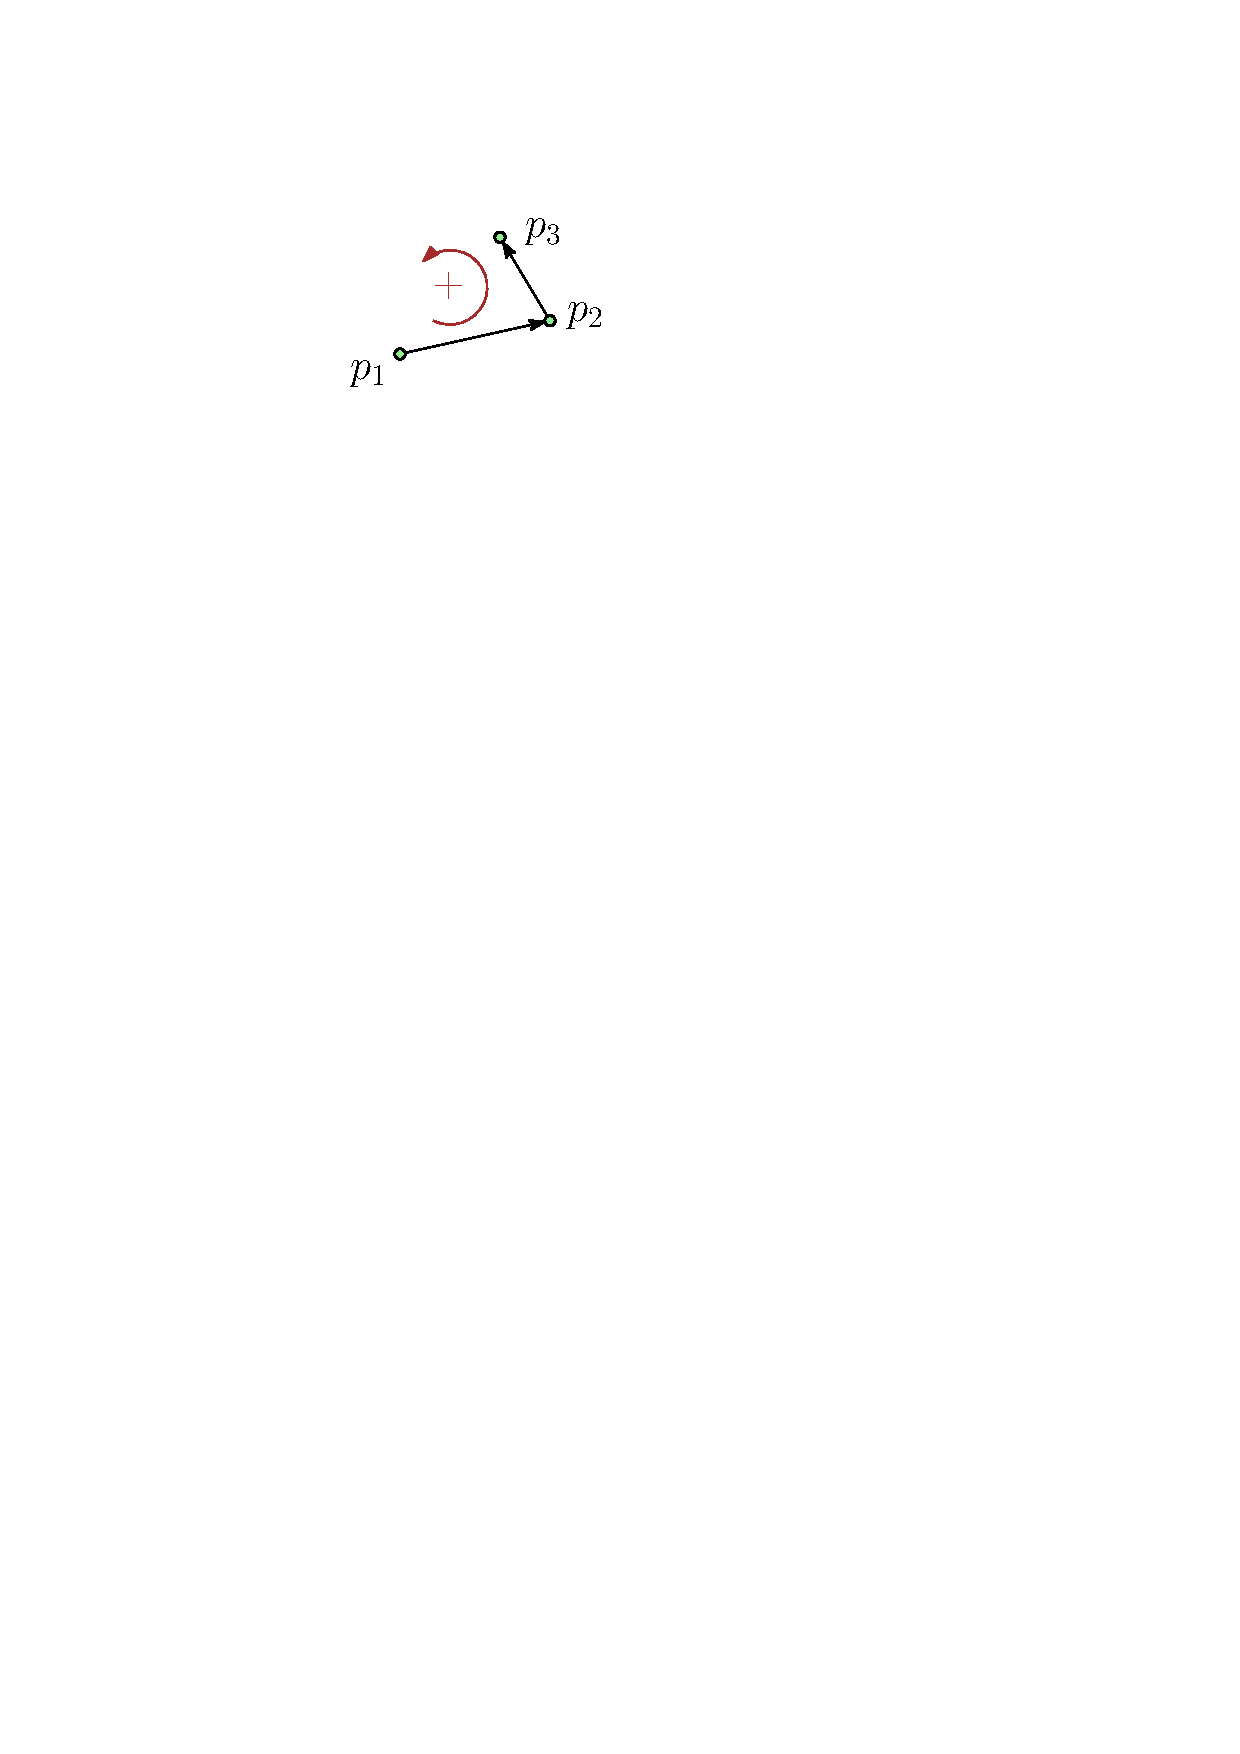
\includegraphics[width=0.13\textwidth]{figures/orientation.pdf}
\end{paracol}
向き$\orient$は三角形の符号付き面積の外積計算そのものである。
従って$\orient$の値が大きいほど$p_3$から$p_1, p_2$を通る直線への垂直距離は大きくなる。
$\orient(p_1, p_2, p_3) = 0$のとき三点は同一直線上にある。
また、$\orient(p_1, p_2, p_3) < 0~(> 0)$のとき右(左)回りもしくは(反)時計回りであり、
$p_3$は$p_1, p_2$を通る直線の右(左)にあるという。
上図は$\orient(p_1, p_2, p_3) > 0$の例を示している。
%おり、($p_1, p_2, p_3)$は反時計回りであり、
%$p_3$は$p_1, p_2$を通る直線の左にある。
%同様に$\orient(p_1, p_2, p_3) < 0$なら$p_3$は右にあるという。





%%%%%%%%%%%%%%%%%%%%%%%%%%%%%%%%%%%%%%%%%%%%%%%%%%%%%%%%%%%%%%%%%%%%%%%%%%%%%%%
\paragraph{タットの平面描画の平面性保証}
タットの平面描画の三制約(外面凸多角形・隣接重心・辺直線分)を満たす描画は、
正しく平面描画になることを示す。
具体的には任意の辺対の写像が交差しないことを議論する。
\begin{theorem}[タットのばね定理]
\label{thm:tutte}
$3$-連結な平面的グラフに対する任意のタットの平面描画は、
どの辺対の写像も交差しない。
\end{theorem}




%%%%%%%%%%%%%%%%%%%%%%%%%%%%%%%%%%%%%%%%%%%%%%%%%%%%%%%%%%%%  Tutte spring theorem.

\begin{proof}%[Proof of \cref{thm:tutte}.]
$p\in \mathbb{R}^2$が
$G$のどの辺の写像にも属さないときファセット上の点と呼ぶ。
ファセット上の点$p$はどれも唯一の面に属すことを示し、
辺対の写像が交差するならその交点の近傍で矛盾が生じることを導く。
外面境界の外部に$p$が属すなら、
タットの平面描画の三つの3制約は外面以外の面に属さないことを保証する。
内部の$p$に対しては
頂点や辺の写像と交差しない半径$\varepsilon ~> 0$の円が描ける。
\cref{lemma:tutte_opposite}より、
任意の辺$e$を共有する二つの面は$e$の写像直線分の左右に分かれるので$p$は唯一の面に属す。
%
%このとき、タットの平面描画の任意の辺対の写像どうしが交差すると仮定すると、
%その交点付近のファセット上の点は二つの面に属すことになり矛盾。
\end{proof}




%%%%%%%%%%%%%%%%%%%%%%%%%%%%%%%%%%%%%%%%%%%%%%%%%%%%%%%%%%%%%%%%%%%%%%% Tutte opposite
\begin{lemma}
\label{lemma:tutte_opposite}
$G=(V, E)$を$3$-連結な平面的グラフ、$\Gamma$を$G$のタットの平面描画とする。
$\ell$を境界上に無い辺$(u, v) \in E$の
端点の写像$p_1=\Gamma(u), p_2=\Gamma(v)$を通る直線とする。
$S_1,~ S_2$をそれぞれ$(u, v)$を共有する二つの面の境界上の$u, v$を除く頂点の集合とする。
%$S_0, S_1$をそれぞれ$F_0, F_1$を構成する$u, v$以外の頂点からなる集合とする。
このとき、$S_1$と$S_2$内の頂点の写像はそれぞれ$\ell$の左右に分かれて存在する。
\end{lemma}

\setcolumnwidth{0.75\textwidth, 0.25\textwidth}
\begin{paracol}{2}
\begin{proof}
$S_1$と$S_2$が$\ell$上か$\ell$の右に存在する
頂点$s_1 \in S_1,~ s_2 \in S_2$をそれぞれ持つと仮定する。
つまり$\orient(p_1, p_2, \Gamma(s_1)) \leq 0$および
$\orient(p_1, p_2, \Gamma(s_2)) \leq 0$。


\cref{lemma:tutte_collinear}および\cref{lemma:tutte_left_right}より、
$s_1,~ s_2$は共に$\ell$の右に写像される隣接頂点を持つ。
\cref{lemma:tutte_connected}より、
経由する頂点がすべて$\ell$の右に写像される$s_1 s_2$-経路$P$が存在する。
%$u,~v$についても同様に、
同様に$u$と$v$はいずれも$\ell$の左に隣接頂点を持ち、
経由する頂点がすべて$\ell$の左に写像される$uv$-経路$Q$が存在する。
\cref{lemma:tutte_left_right}より$Q$は$(u, v)$でない。
また$P$と$Q$は互いに点素。
これは\cref{lemma:tutte_cycle_intersection}に矛盾する。
\end{proof}
\switchcolumn
%\vspace{1.5\intextsep}
\centering
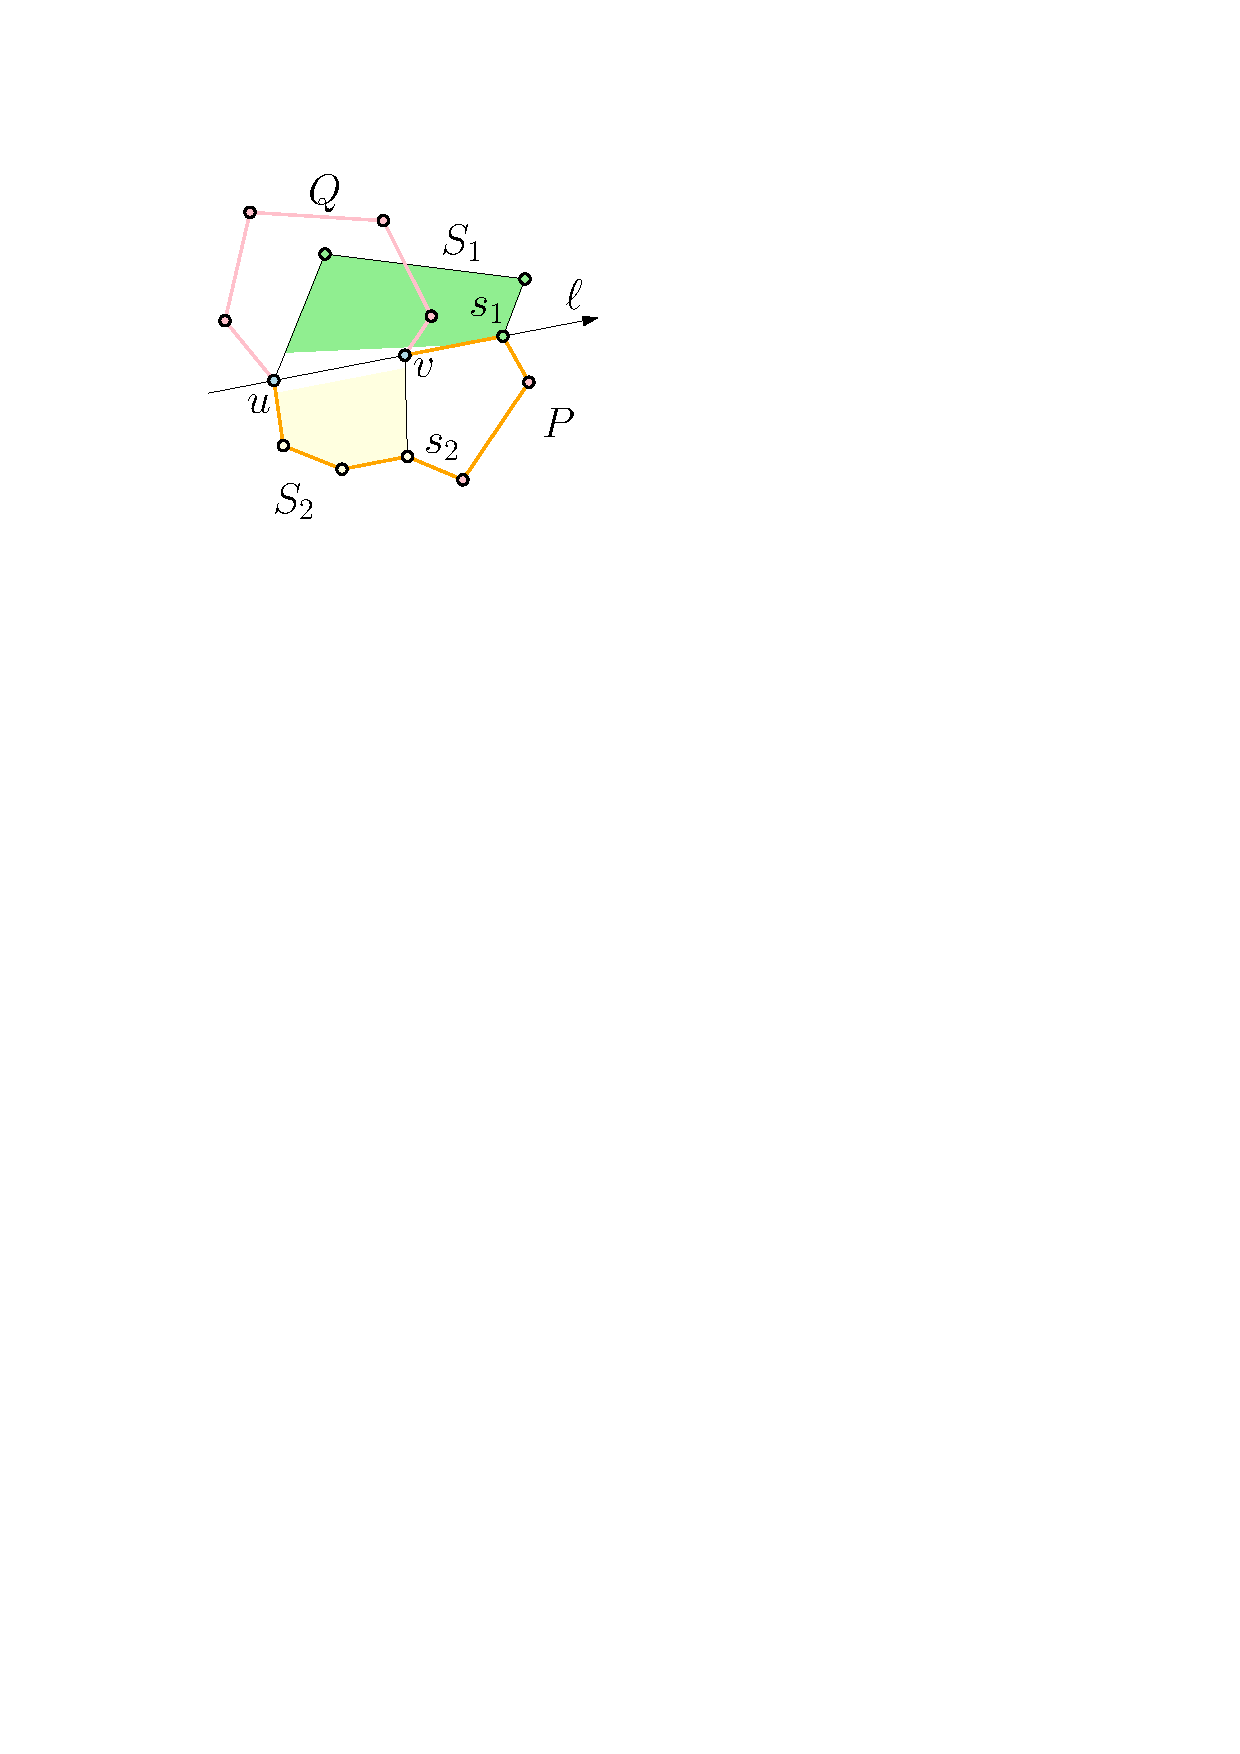
\includegraphics[width=0.2\textwidth]{figures/tutte_opposite.pdf}
\end{paracol}





%%%%%%%%%%%%%%%%%%%%%%%%%%%%%%%%%%%%%%%%%%%%%%%%%%%%%%%%%%%%%%%%%%%%%%% Tutte collinear
\begin{lemma}
\label{lemma:tutte_collinear}
隣接頂点すべての写像が同一直線上に配置される頂点は存在しない。
\end{lemma}

\setcolumnwidth{0.75\textwidth, 0.25\textwidth}
\begin{paracol}{2}
\begin{proof}
%外面境界上の頂点集合$F$に関しては前提条件。
すべての隣接頂点が直線$\ell$上に位置する頂点$v$が存在すると仮定する。
$S^+,~ S^-$をそれぞれ$\ell$の左と右に写像を持つ頂点の集合とする。
$U$を$v$から到達可能な頂点$u$で$N(u)$がすべて$\ell$上に写像される頂点集合とする。
少なくとも$v \in U$。
$W$を$v$から到達可能で$\ell$上に写像されるが$S^+,~ S^-$に隣接頂点を持つ頂点の集合とする。
\cref{lemma:tutte_left_right}より$W\neq \varnothing$。
また、対象グラフは$3$-連結であり、
$W$は$U$と$S^+\cup S^-$に対する切断集合なので$|W|\geq 3$。
%$W$の各頂点は$S^+$と$S^-$両方に隣接頂点を持つ。
\cref{lemma:tutte_connected}より$S^+$と$S^-$はそれぞれ連結である。
$w_1, w_2, w_3 \in W$および$S^+, U, S^-$は$K_{3,3}$の細分を形成する。
\end{proof}
\switchcolumn
\vspace{-1.5\intextsep}
\centering
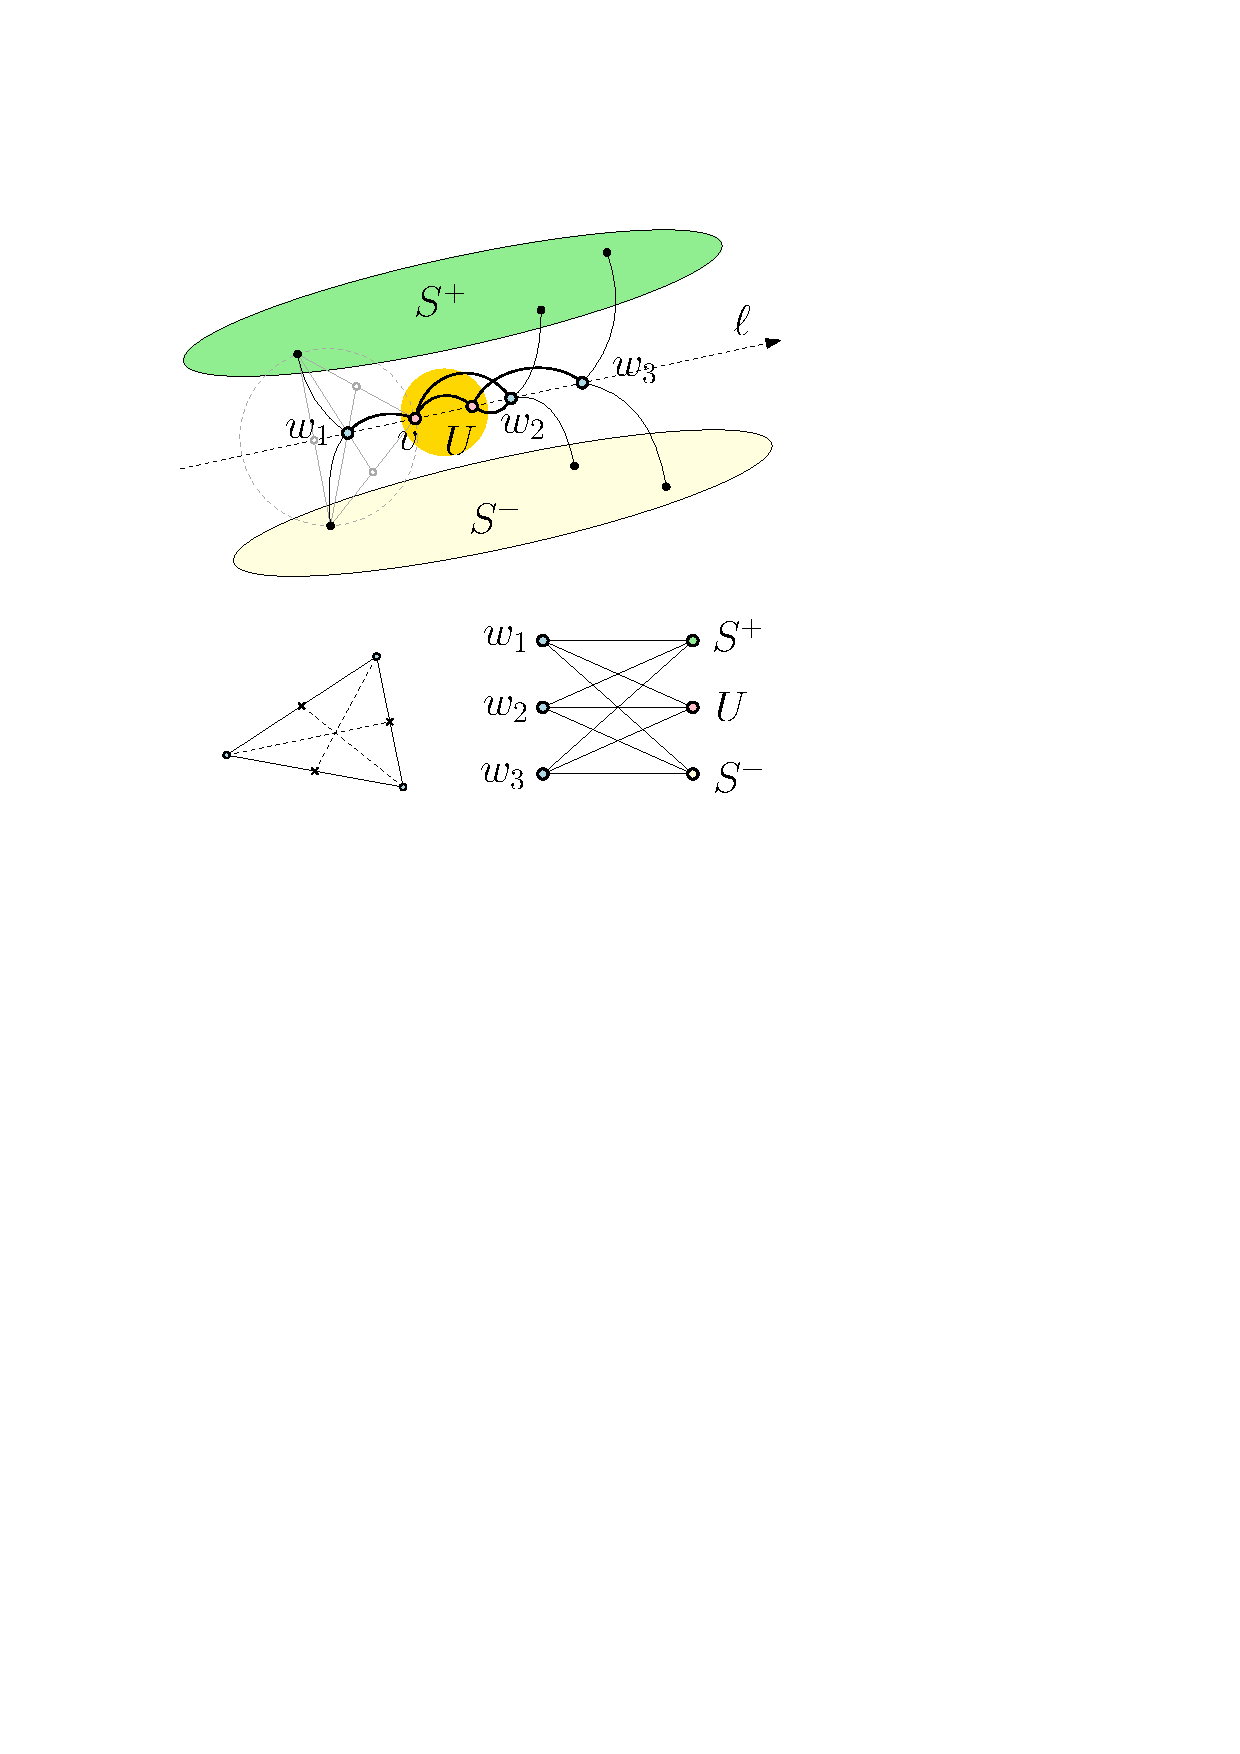
\includegraphics[width=0.24\textwidth]{figures/tutte_collinear.pdf}
\end{paracol}










\begin{lemma}
\label{lemma:tutte_left_right}
$\ell$をある頂点$v \in V$の写像$p_1 = \Gamma(v)$と
任意の点$p_2 \in \mathbb{R}^2$を通る直線とする。
$\ell$の左に位置する$v$の隣接頂点が非空
$\{u \in N(v) ~|~ \orient(p_1, p_2, \Gamma(u)) > 0\} \neq \varnothing$なら
右の隣接頂点も非空$\{u \in N(v) ~|~ \orient(p_1, p_2, \Gamma(u)) < 0\} \neq \varnothing$。
\end{lemma}

\begin{proof}
任意の内部頂点は、
第2制約により各$xy$-座標の平均値をとるので、
隣接頂点の写像が形成する凸包の外部に位置することはない。
\end{proof}


%%%%%%%%%%%%%%%%%%%%%%%%%%%%%%%%%%%%%%%%%%%%%%%%%%%%%%%%%%%%%%%%%%%%%%%%%%コメントアウト
\begin{comment}
\begin{lemma}
外面境界上の頂点集合$F$に無いすべての頂点は$F$の凸包内部$C$に含まれる。
\end{lemma}

\begin{proof}
外面境界上の点集合の任意の$3$点$v_1, v_2, v_3$からなる集合を$A$、$B=\{v\}$とするとき
メンガーの\cref{thm:menger}より$v$から$v_i,~ i=1,2,3$への点素経路を持つ。
$\Gamma(v)$は$\Gamma(v_i), i=1,2,3$の加重平均と見做せるので
$C$の境界上ではない内部に配置される。
\end{proof}
\end{comment}
%%%%%%%%%%%%%%%%%%%%%%%%%%%%%%%%%%%%%%%%%%%%%%%%%%%%%%%%%%%%%%%%%%%%%%%%%%コメントアウト



\begin{lemma}
\label{lemma:tutte_connected}
$G=(V,E)$を対象のグラフ、$\Gamma$を任意のタットの平面描画、
$H$を任意の$2$点$p_1, p_2 \in \mathbb{R}^2,~ p_1\neq p_2$を通る直線で区切られる
半平面$\{p \in \mathbb{R}^2 ~|~ \orient(p_1, p_2, p) > 0\}$とする。
%このとき
$S = \{v \in V~|~ \Gamma(v)\in H\}$が誘導する部分グラフ$G[S]$は連結。
\end{lemma}

\vspace*{-0.5\intextsep}
\setcolumnwidth{0.78\textwidth, 0.22\textwidth}
\begin{paracol}{2}
\begin{proof}
平面上の点$p\in \mathbb{R}^2$に対して$\tau(p) = \orient(p_1, p_2, p)$とおく。
$F$を外面境界上の頂点集合とする。
$H$の境界線から最も離れた頂点$t = \argmax_{v\in V}\tau(\Gamma(v))$は$t\in F$。
任意の頂点$s\in S$から$t$への経路$s=v_0, v_1, \ldots, v_k=t$で
連続する二頂点$v_i, v_{i+1}$が
$\tau(\Gamma(v_i)) \leq \tau(\Gamma(v_{i+1}))$ を満たす経路が存在することを示す。

$p=\Gamma(s),~ q=\Gamma(t)$とおく。
$\tau(p) = \tau(q)$のとき
$s$と$t$はいずれも$F$内の頂点で互いに隣接する。
%これは$p_1, p_2$および$p, q$それぞれの方向ベクトルが平行で、すなわち
%符号付き面積が等しくなることを意味する。
%
$\tau(p) < \tau(q)$のとき二つの場合を考える。
%$s$から$t$への$\tau$が非減少の経路が存在することを示す。
$s \in F$なら外面境界を辿り$t$へ到達する経路が存在する。
$s \notin F$なら\cref{lemma:tutte_left_right}より、
$\tau(p) < \tau(\Gamma(v))$を満たす$v \in N(s)$が存在する。
これは帰納的に成り立ち、$S$の任意の頂点は$t$へ到達可能。
\end{proof}
\switchcolumn
\vspace{1.5\intextsep}
\centering
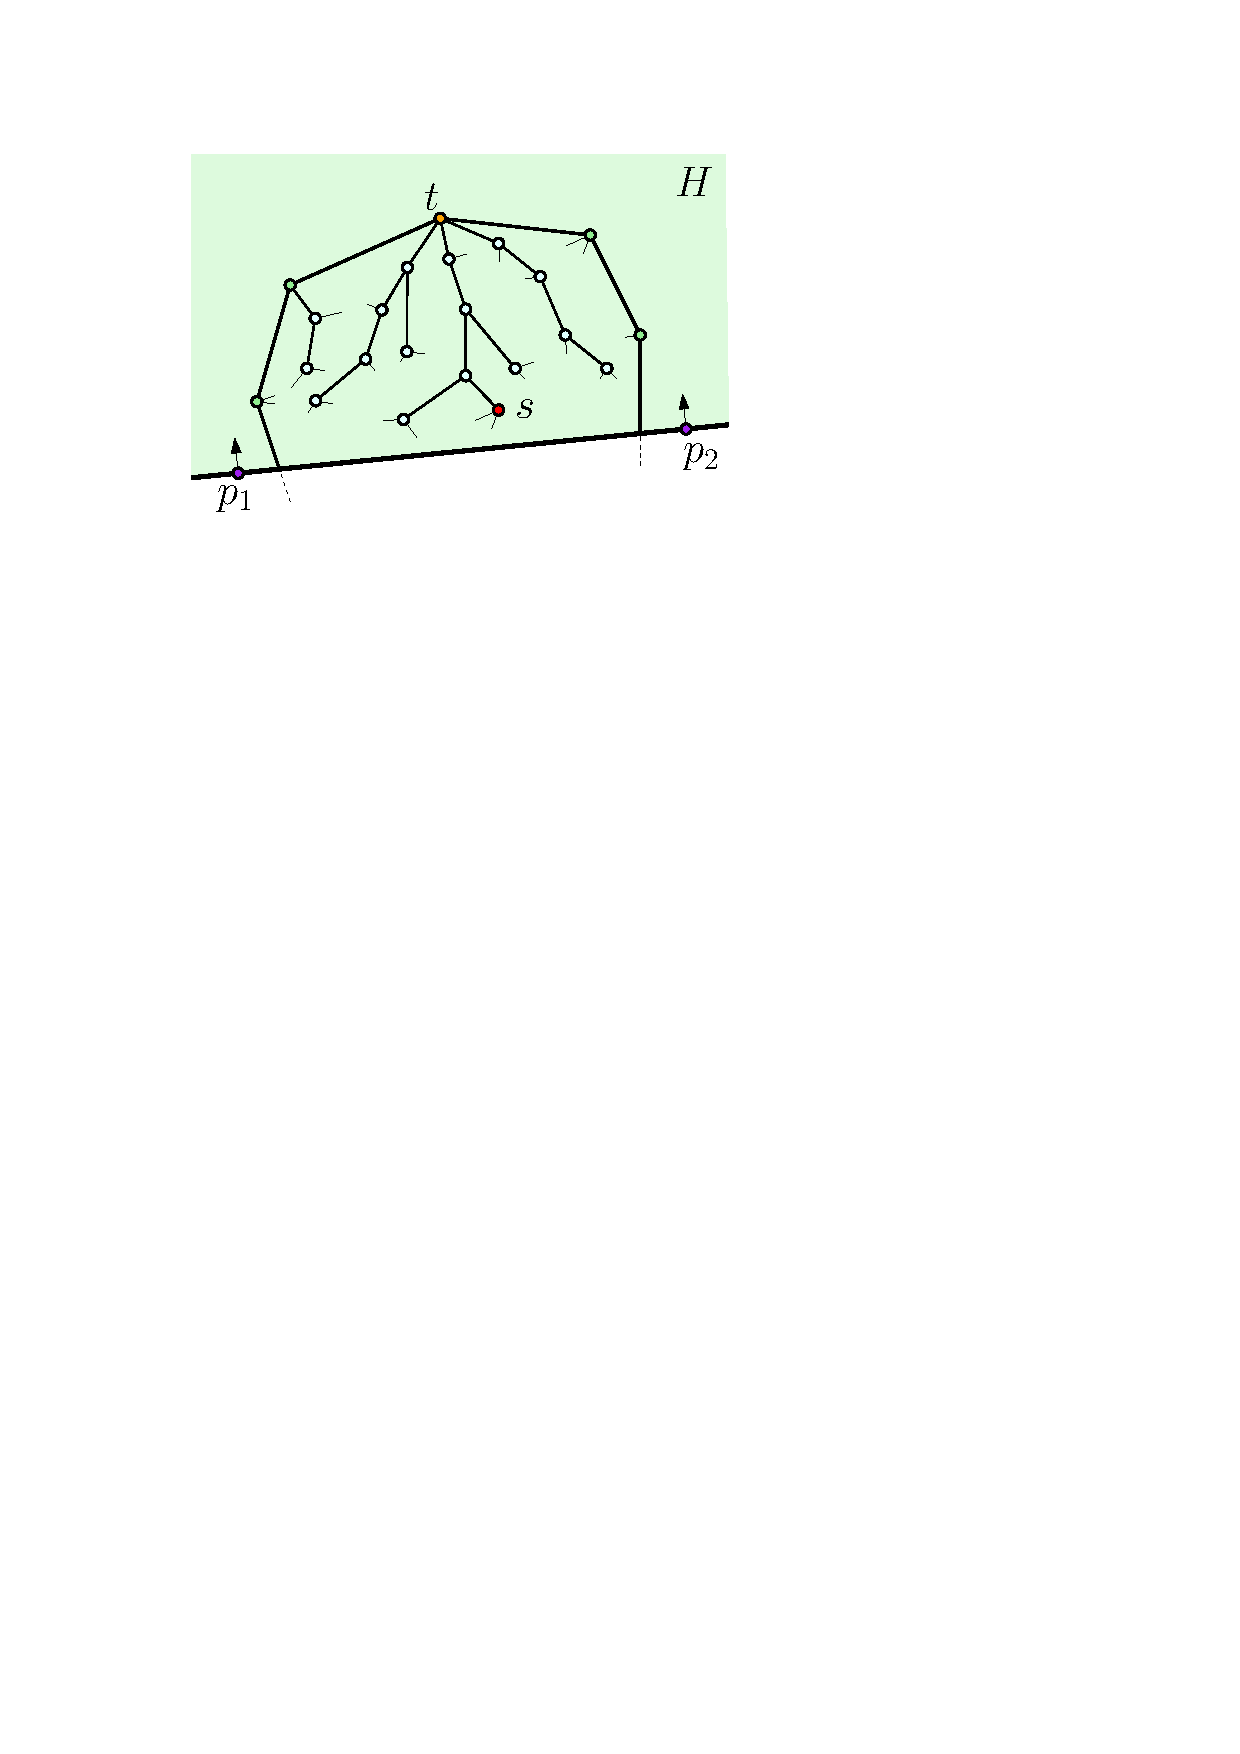
\includegraphics[width=0.21\textwidth]{figures/tutte_connected.pdf}
\end{paracol}




\setcolumnwidth{0.75\textwidth, 0.25\textwidth}
\begin{paracol}{2}
\begin{lemma}
\label{lemma:tutte_cycle_intersection}
$G$を$3$-連結な平面的グラフ、$(u, v)$を$G$の任意の辺とする。
$S_1, S_2$をそれぞれ$(u, v)$を共有する面の$u, v$を除く頂点集合とする。
$P$をその端点が$s_1 \in S_1,~ s_2 \in S_2$で$u, v$を経由しない$G$上の経路とする。
このとき、$G$上の任意の$uv$-経路は$P$と共通頂点を持つか$(u, v)$自身である。
\end{lemma}


\begin{proof}
$G$の任意の平面描画を考える。
このとき$P$と$s_1, s_2$を仮想的につなげたジョルダン閉曲線$C$が描ける。
$C$の仮想的な部分曲線は$(u, v)$の写像とだけ交差し、$u$と$v$を内と外に分かつ。
従って、$u$と$v$を端点とするどんな経路も$P$と少なくとも一つの頂点を共有するか
辺$(u, v)$そのものである。
\end{proof}
\switchcolumn
\vspace{1.\intextsep}
\centering
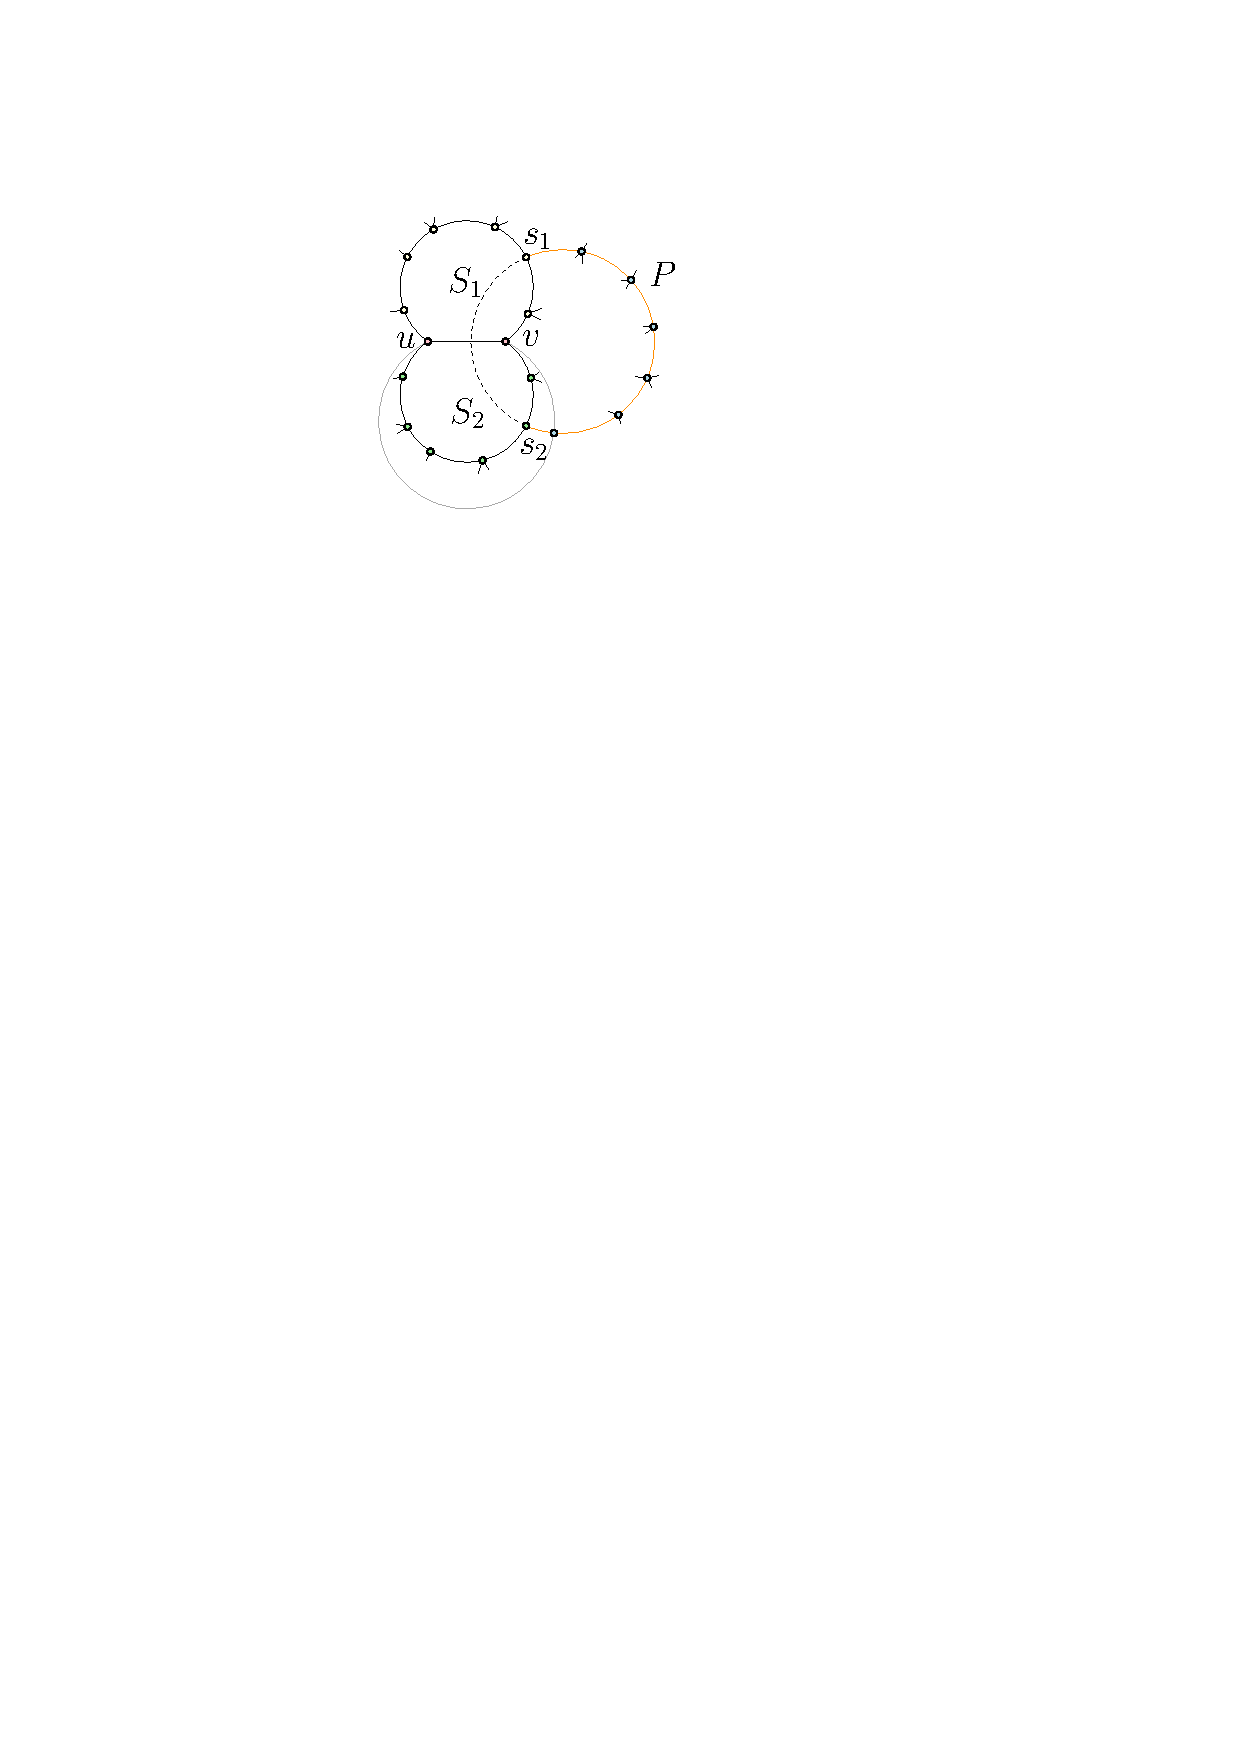
\includegraphics[width=0.21\textwidth]{figures/tutte_cycle_intersection.pdf}
\end{paracol}


%%%%%%%%%%%%%%%%%%%%%%%%%%%%%%%%%%%%%%%%%%%%%%%%%%%%%%%%%%%%%%%%%%%%%%%%コメントアウト
\begin{comment}
\paragraph{タットのばね\cref{thm:tutte}からの系}
以降のクラトフスキー定理の証明および平面性判定で用いる
タットのばね\cref{thm:tutte}の系を記述する。


\begin{corollary}
\label{coro:convex_face}
タットの平面描画の各面はいずれも凸多角形。
\end{corollary}


\begin{corollary}
\label{coro:tutte_any_face}
平面的グラフ$G$は任意の頂点を外面に持つ平面埋込みを持つ。
\end{corollary}

\cref{coro:convex_face}は
\cref{lemma:tutte_opposite}および\cref{lemma:tutte_collinear}によって保証される。
タットの平面描画は平面埋込みからの面選択に制限を課さないので
\cref{coro:tutte_any_face}は、
$1$-連結や$2$-連結なグラフであっても仮想的に辺を追加して$3$-連結にしてから
タットの平面描画を実行すると任意の包囲閉路を外面とする平面描画が得られる。
\end{comment}
%%%%%%%%%%%%%%%%%%%%%%%%%%%%%%%%%%%%%%%%%%%%%%%%%%%%%%%%%%%%%%%%%%%%%%%%コメントアウト










%%%%%%%%%%%%%%%%%%%%%%%%%%%%%%%%%%%%%%%%%%%%%%%%%%%%%%%%%%%%%%%%%%%%%%%%%%%%%%%%%%%%%%%
\subsection{クラトフスキーの定理}
\label{subsec:kuratowski}

\setcolumnwidth{0.66\textwidth, 0.33\textwidth}
\begin{paracol}{2}
ここではクラトフスキーの定理を考察する。
特にグラフが非平面的なら必ずクラトフスキー部分グラフを持つことを示す。


\begin{theorem}[クラトフスキー定理]
\label{thm:kuratowski}
グラフ$G$が平面的であることの必要十分条件は
$G$が部分グラフとして$K_5$もしくは$K_{3,3}$の細分を持たないこと。
\end{theorem}

\switchcolumn
%\vspace{1.5\intextsep}
\centering
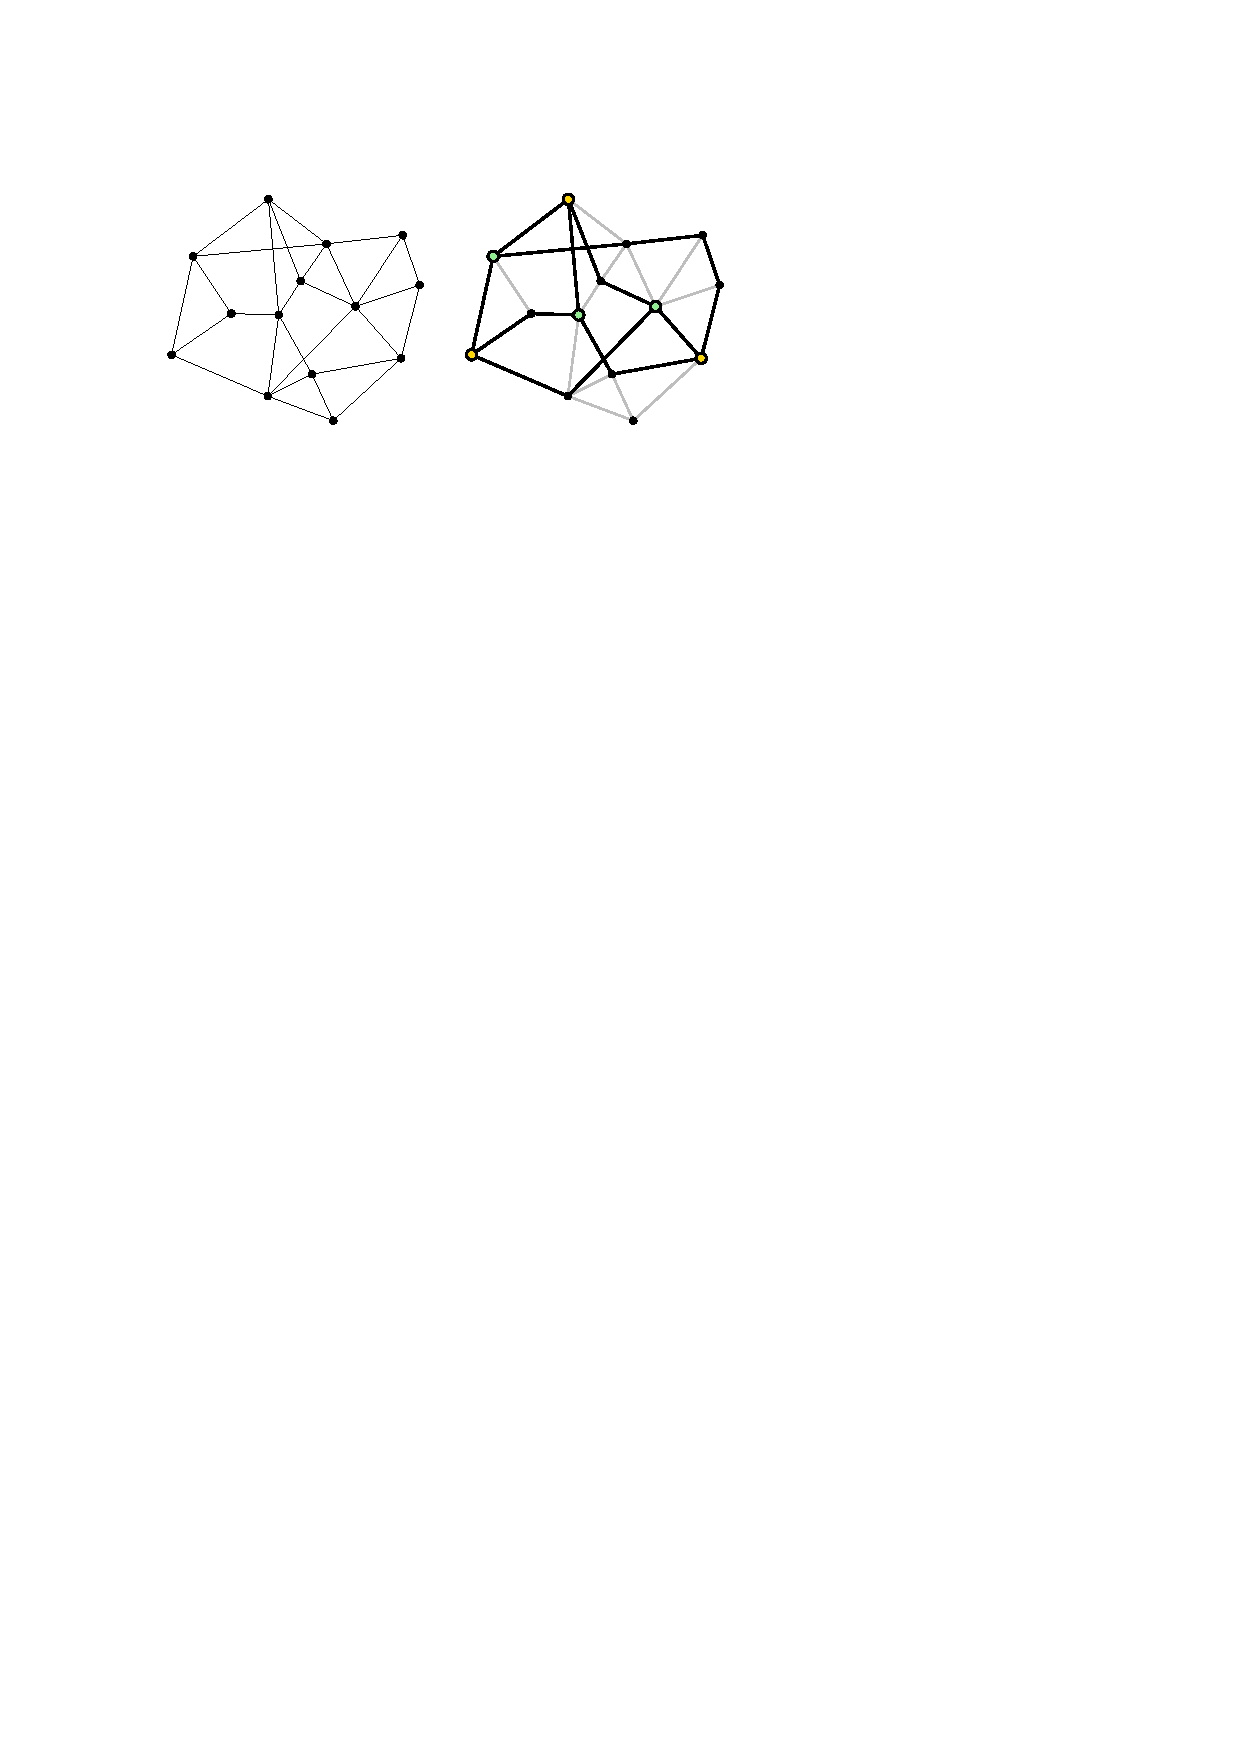
\includegraphics[width=0.3\textwidth]{figures/kuratowski_subgraph_example_01.pdf}
\end{paracol}

\paragraph{十分性の証明}
必要性はオイラーの多面体公式の\cref{coro:girth}および
辺細分による頂点数と辺数の増分差分の不変性を確認すれば帰納的に示せる。
%以下では十分性を証明する。
以下では極小な非平面的グラフを対象に議論する。
これは、どんな非平面的グラフも辺を削除していけば最終的に平面的になり、
その直前には近傍に極小性を有する部分グラフが存在することから
一般性を失わない。



\begin{lemma}[クラフトスキーの定理の十分性]
グラフ$G$が非平面的ならクラトフスキー部分グラフを持つ。
\end{lemma}

\begin{proof}
\cref{lemma:3_connectivity} は、
クラトフスキー部分グラフを持たない辺数最小の非平面的グラフが存在するなら
それは$3$-連結であることを保証する。
また、\cref{lemma:contractions_dont_make_kuratowski_subgraph}および
\cref{lemma:contractions_preserve_3_connectivity} は、
$3$-連結性を保持しつつクラトフスキー部分グラフを生成しないよう
極小非平面的グラフの辺数を可能な限り減らすことができることを保証する。
一方で\cref{lemma:tutte} は、
クラトフスキー部分グラフを持たない$3$-連結なグラフには
平面描画が存在することを保証する。
これは極小な非平面的グラフが
クラトフスキー部分グラフを持つことの証左である。
\end{proof}



%以下では極小な非平面的グラフに限定して議論する。
%頂点や辺の追加によって非平面的なグラフが平面的になったり
%クラトフスキー部分グラフが消失することはないため、
%極小なグラフに限定しても一般性を失わない。



%%%%%%%%%%%%%%%%%%%%%%%%%%%%%%%%%%%%%%%%%%%%%%%%%%%%%%%%%%%%%%%%%%%%%%%%%%%%% Lemma 2
\begin{lemma}\label{lemma:1-connected}
極小な非平面的グラフは$1$-連結。
\end{lemma}

\begin{proof}
$1$-連結でないと仮定する。
いずれの成分も非平面的なら任意の辺削除で平面的とならず極小性に反する。
同様に平面的な連結成分が存在するならその成分内の辺を削除しても平面的とはならない。
\end{proof}


%%%%%%%%%%%%%%%%%%%%%%%%%%%%%%%%%%%%%%%%%%%%%%%%%%%%%%%%%%%%%%%%%%%%%%%%%%%%% Lemma 3
\begin{lemma}\label{lemma:2-connected}
極小な非平面的グラフは$2$-連結。
\end{lemma}

\begin{proof}
$2$-連結でない、つまり切断点$v$を持つ極小な非平面的グラフ $G=(V, E)$ が存在すると仮定する。
$C \subseteq V$ を $G \setminus v$ の任意の連結成分の頂点集合とする。
このとき誘導部分グラフ$G[C \cup \{v\}]$および$G \setminus C$は
互いに辺素なので
\cref{lemma:1-connected} の証明と同様の議論により極小性に反する。
\end{proof}



%%%%%%%%%%%%%%%%%%%%%%%%%%%%%%%%%%%%%%%%%%%%%%%%%%%%%%%%%%%%%%%%%%%%%%%%%%%%%%%%%%% Lemma 4
\begin{lemma}\label{lemma:edge_disconnected}
$G=(V, E)$ を非平面的グラフとする。
$x, y \in V$ を $G' = G \setminus \{x, y\}$ が非連結となる頂点対とする。
このとき、次を満たす $G'$ の連結成分$C \subseteq V$ が存在する。
$C \cup \{x, y\}$ および辺 $(x, y)$ が誘導する部分グラフが非平面的。
\end{lemma}

\vspace*{-\intextsep}
\setcolumnwidth{0.8\textwidth, 0.2\textwidth}
\begin{paracol}{2}
\begin{proof}
$C_1, \ldots, C_k$ を $G'$ の連結成分とする。
$G'_i$ を $C_i \cup \{x, y\}$ に辺$(x,y)$を加えて誘導される部分グラフとする。
各 $G'_1, \ldots, G'_k$ はいずれも平面的と仮定する。
このとき$H_1$ を $G'_1$ の平面描画とすると、
$2 \leq i \leq k$ に関して $H_{i-1}$ の $(x, y)$ を含むいずれかの面の内部に
$G'_i$ を描画して得られる平面描画 $H_i$ が存在する。
帰納的に$H_k - (x, y)= G$ は平面的であるがこれは主張の前提に反する。
\end{proof}

\switchcolumn
%\begin{figure}[ht]
\centering
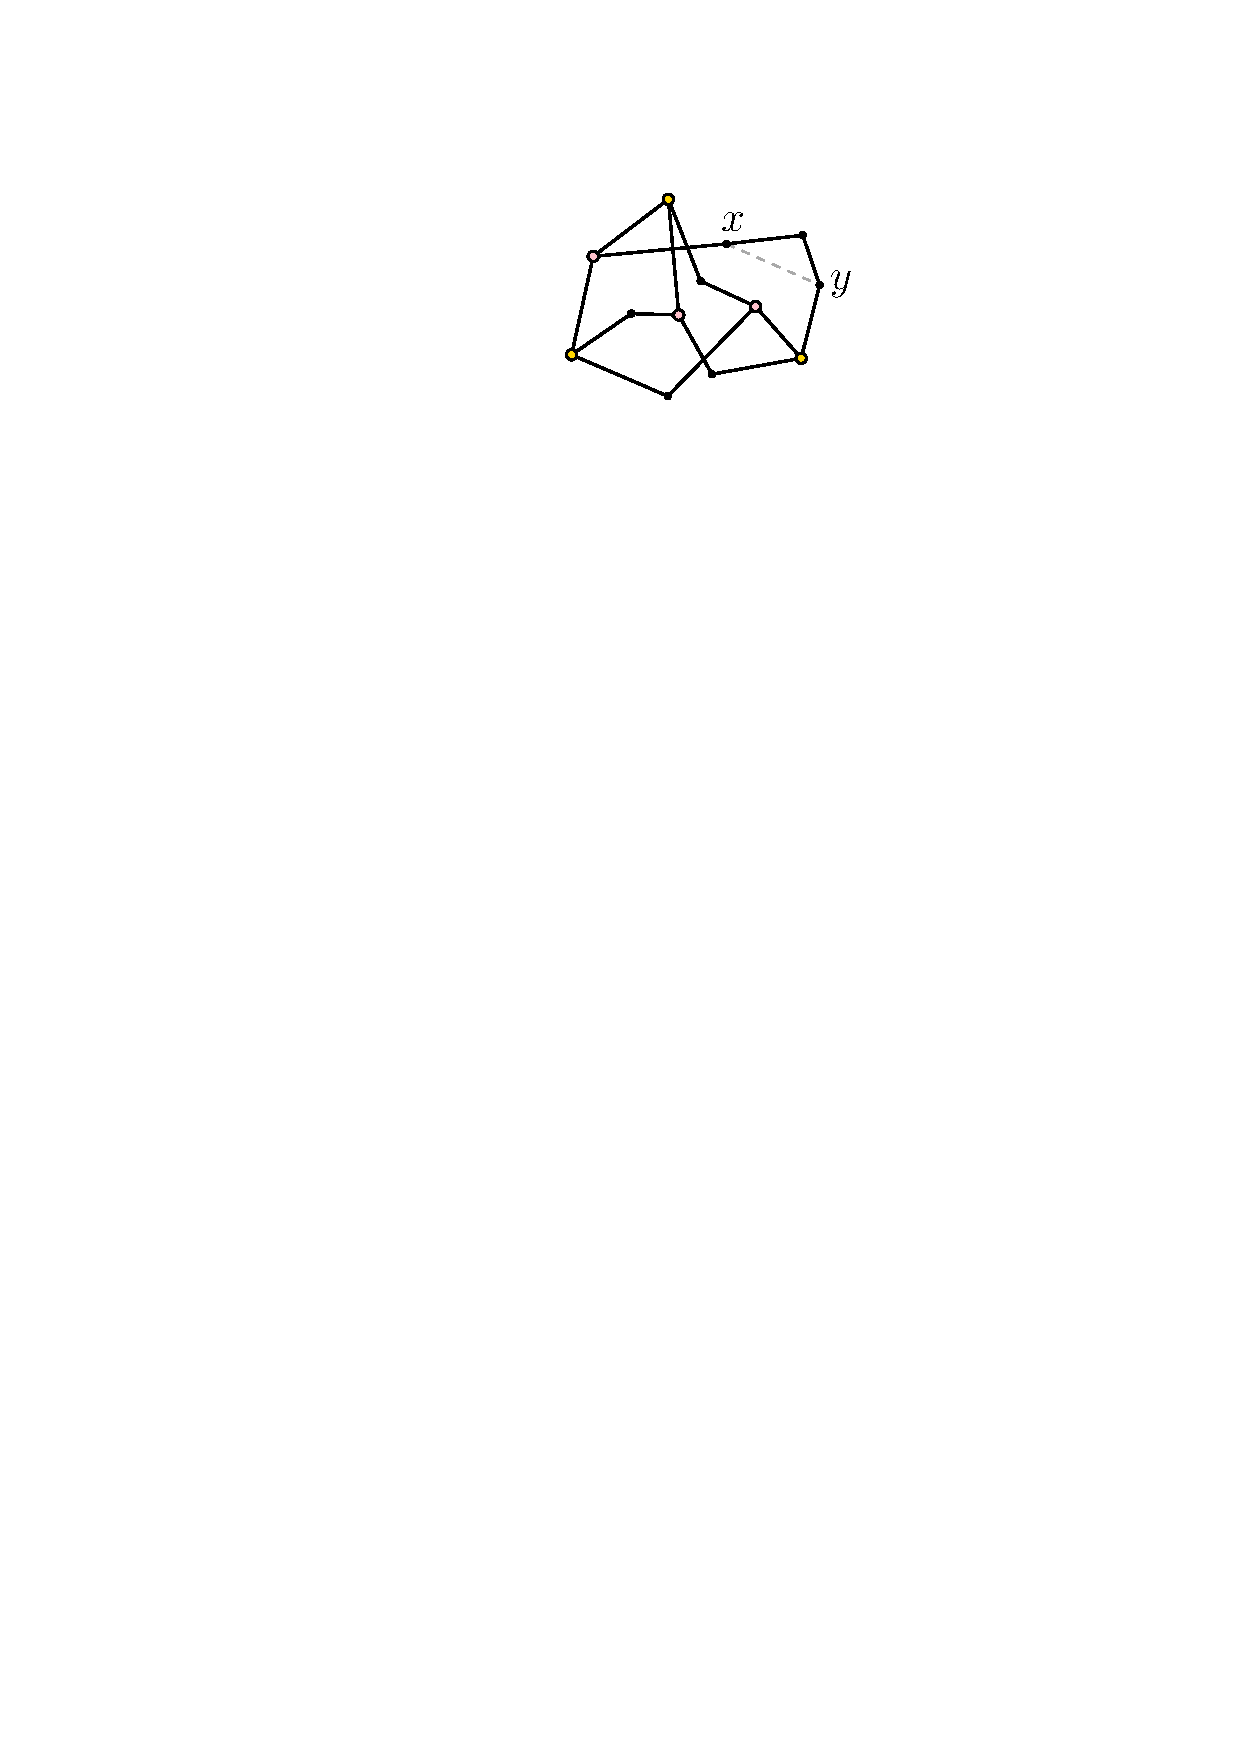
\includegraphics[width=0.18\textwidth]{figures/kuratowski_subgraph_example_02.pdf}
%\end{figure}
\end{paracol}


%%%%%%%%%%%%%%%%%%%%%%%%%%%%%%%%%%%%%%%%%%%%%%%%%%%%%%%%%%%%%%%%%%%%%%%%%%%%%%%%% Lemma 5
\begin{lemma}\label{lemma:3_connectivity}
$G = (V, E)$ をクラトフスキー部分グラフを持たない
すべての非平面的グラフの中で辺数最小のグラフとするなら、
$G$は$3$-連結。
\end{lemma}

\begin{proof}
$G$は極小なので\cref{lemma:2-connected}~より$2$-連結。
$G$ を非連結にする二頂点 $x, y \in V$ が存在すると仮定すると、
$G\setminus \{x, y\}$ は連結成分 $C_1, \ldots, C_k$ を持つ。
\cref{lemma:edge_disconnected} より
$C_i \cup \{x, y\}$ に辺 $(x,y)$を加えて誘導される部分グラフ $H$ が
非平面的となる $C_i$ が存在する。
$G$ の辺数最小性より $H$ はクラトフスキー部分グラフ $K$ を持つが、
$(x, y) \notin E$なので $K$ は $G$ の部分グラフではない。
$G$は$2$-連結なので、メンガーの\cref{thm:menger}より、
別の連結成分 $C'$ の頂点のみで構成される $x$ と $y$ をつなぐパス $P$ が存在する。
$K$ と $P$ をつなぎ合わせると$G$内にクラフトスキー部分グラフを得る。
\end{proof}


%%%%%%%%%%%%%%%%%%%%%%%%%%%%%%%%%%%%%%%%%%%%%%%%%%%%%%%%%%%%%%%%%%%  Menger

\begin{comment}
上記の証明では暗にメンガーの定理を利用している。

\begin{theorem}[メンガーの定理]
グラフが$k$-連結である必要十分条件は、任意の二頂点間に$k$個の点素パスが存在すること。
\end{theorem}
\end{comment}


%%%%%%%%%%%%%%%%%%%%%%%%%%%%%%%%%%%%%%%%%%%%%%%%%%%%%%%%%%%%%%%%%%%%%%%%%% Lemma 6
\begin{lemma}\label{lemma:contractions_dont_make_kuratowski_subgraph}
$G = (V, E)$ をクラトフスキー部分グラフを持たないグラフとする。
任意の辺 $e \in E$ を縮約してもクラフトスキー部分グラフにはならない。
\end{lemma}

\vspace*{-\intextsep}
\setcolumnwidth{0.7\textwidth, 0.3\textwidth}
\begin{paracol}{2}
\begin{proof}
$G / e$と$v_e$をそれぞれ$e=(x, y) \in E$ を縮約して得られるグラフと頂点とする。
$G/e$ がクラトフスキー部分グラフ$H$を持つと仮定する。
%頂点 $v_e$ を辺$e$を縮約して得られる頂点とし次数を$d(v_e)$とする。
$v_e$ が $H$ の頂点でないなら $H$は$G$の部分グラフとなり矛盾。
$H$の最小次数は$2$、最大次数は$4$なので $2 \leq \deg(v_e) \leq 4$。
$\deg(v_e) = 2$なら$x$と$y$の縮約前の次数の組合せは、
$\deg(x) = \deg(y) = 2$もしくは一方が$1$か$3$の場合である。
いずれも$G$は$H$の細分か同型な部分グラフを持つこととなり矛盾。
$\deg(v_e)\geq 3$で$x, y$のいずれかの次数が$\deg({v_e})$以上の場合、
$H$の細分は$G$の部分グラフとなるので矛盾(右図上段)。
$H$が$K_5$の細分であり、$\deg(x) = \deg(y) = 3$の場合、
$G$は$K_{3,3}$の細分を持つので矛盾(右図下段)。
\end{proof}


\switchcolumn
%\begin{figure}[h]
\vspace{0.5\intextsep}
\centering
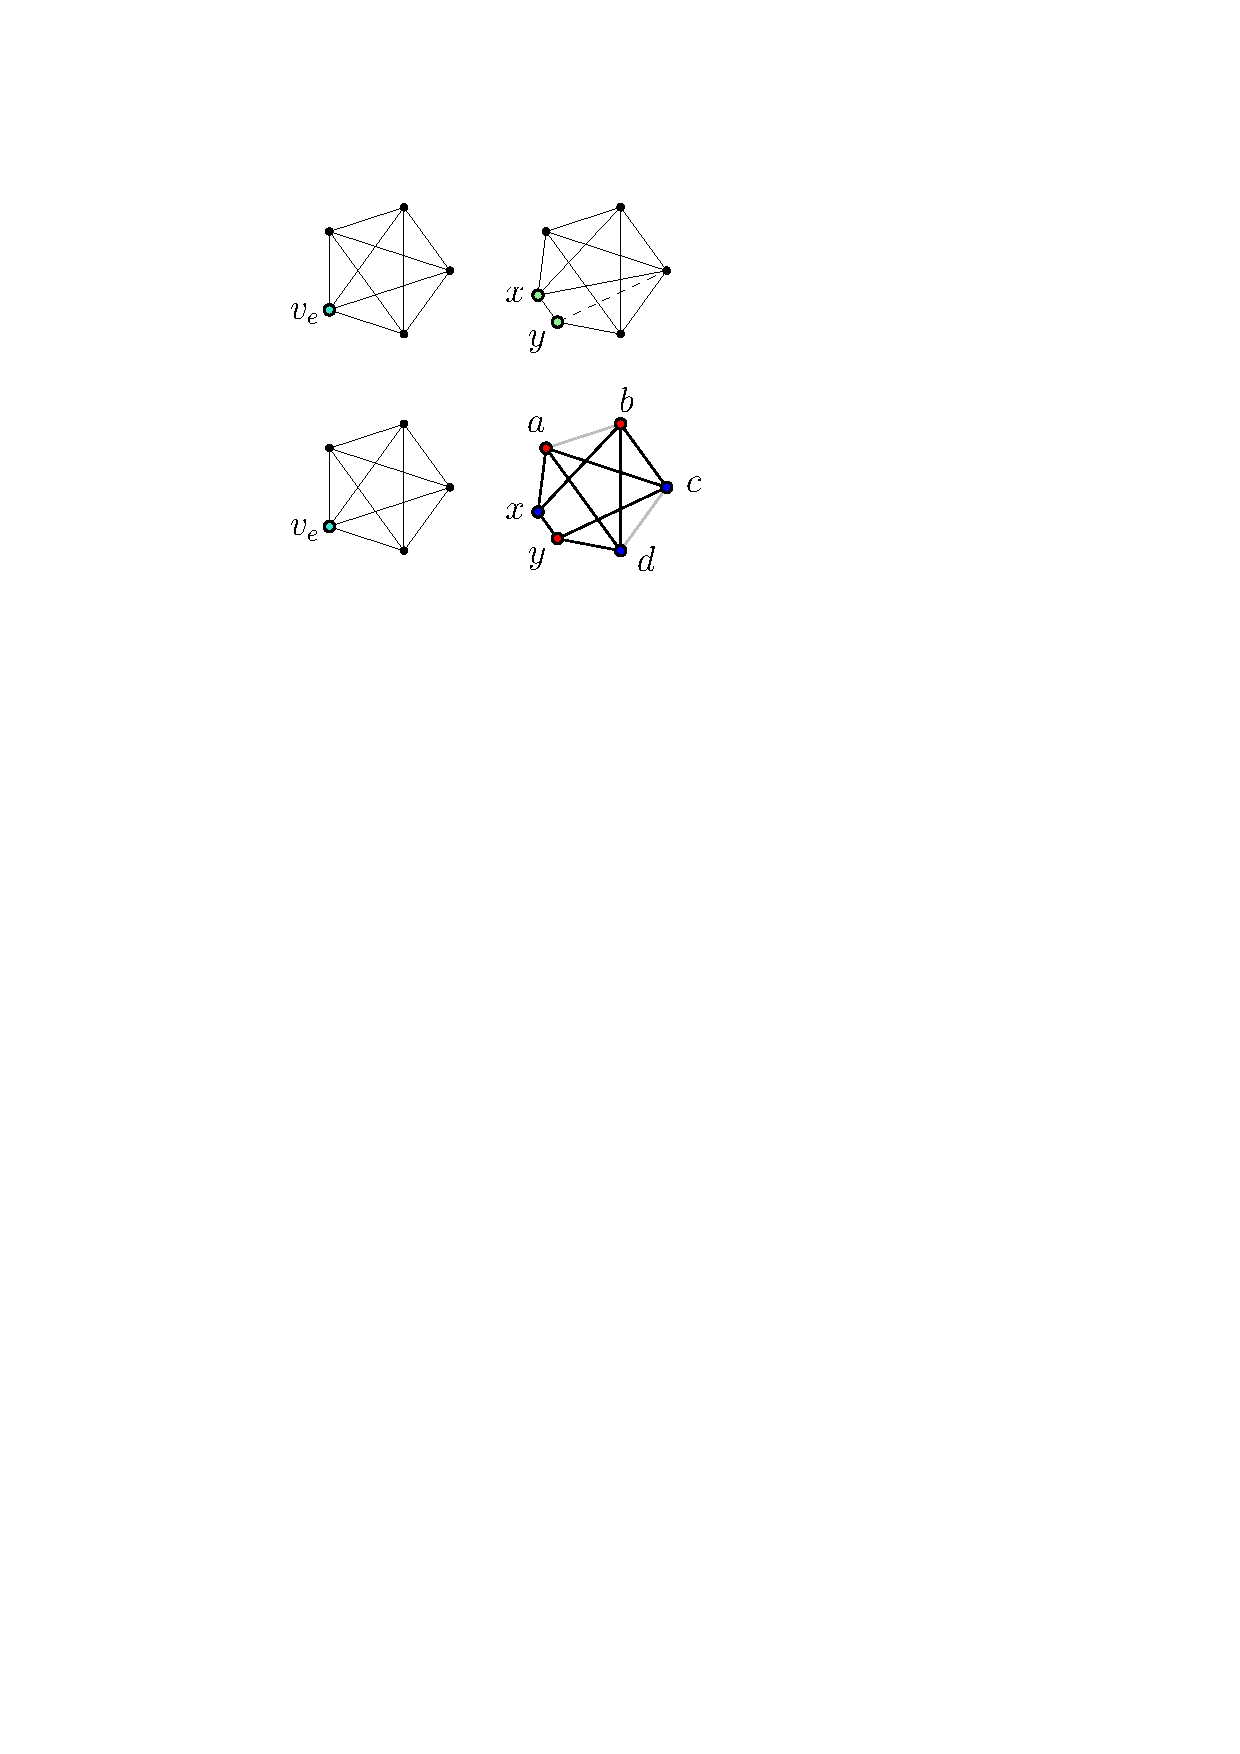
\includegraphics[width=0.25\textwidth]{figures/contraction_01.pdf}
%\end{figure}
\end{paracol}



%%%%%%%%%%%%%%%%%%%%%%%%%%%%%%%%%%%%%%%%%%%%%%%%%%%%%%%%%%%%%%%%%%%%%%%%%%%%%%%%%% Lemma 7
\begin{lemma}\label{lemma:contractions_preserve_3_connectivity}
$G = (V, E)$ を$|V| \geq 5$の$3$-連結なグラフとする。
$G$ は縮約しても$3$-連結性を損なわない辺を持つ。
\end{lemma}



\vspace*{-\intextsep}
\setcolumnwidth{0.75\textwidth, 0.25\textwidth}
\begin{paracol}{2}
\begin{proof}
どの辺$e\in E$を縮約対象に選んでも$3$-連結性を損なう$G$が存在すると仮定する。
このとき、どの辺$e=(x, y)$にも
$G \setminus \{x, y, \delta(e)\}$で非連結になる頂点$\delta(e)\in V$が存在する。
$C_e$を$G \setminus \{x, y, \delta(e)\}$内で頂点数最大の連結成分の頂点集合とする。
%
%$v_e$を$e$の縮約で生成される頂点とすると$G / e \setminus \{v_e, \delta(e)\}$が
%非連結となる頂点$\delta(e) \in V$が存在する。
%$G'=G/e$とし$v_e$を$e$を縮約して得られる頂点とする。
%任意の$e=(x, y)\in E$に関して$G'$が$3$-連結ではないと仮定すると
%$G'\setminus \{v_e, z_e\}$が非連結となる頂点$z_e\in V$が存在し、
%$\{x, y, z_e\}$の削除で$G$は非連結となる。
%任意の辺$e=(x, y)$に対して
%
%任意の辺$e=(x, y)$が与えられたとき
%$C_e$ を$G \setminus \{x, y, z_e\}$内の最も大きな連結成分とする。
%$C_e$ は背理法の仮定の下で well-defined。
%以下、
$e^* = \argmax_{e \in E} (|C_e|)$とする。
$C'$を$G\setminus \{x, y, \delta(e^*)\}$の$C_{e^*}$以外の連結成分とする。
$G$は$3$-連結なので$\delta(e^*)$と$u \in C'$を接続する辺$f$が存在する。
$f$についても同様に$G$を非連結にする頂点$\delta(f)$が存在する。
$G[C_{e^*} \cup \{x, y\}]$は$2$-連結で$\delta(f)$を削除しても連結性を失わないので
$G\setminus \{\delta({e^*}), u, \delta(f)\}$は少なくとも頂点数
$|C_{e^*} \cup \{x, y\}|-1$の連結成分を持つが、これは$C_{e^*}$の最大性に矛盾する。
\end{proof}

\switchcolumn
\vspace{1\intextsep}
%\begin{figure}[ht]
\centering
%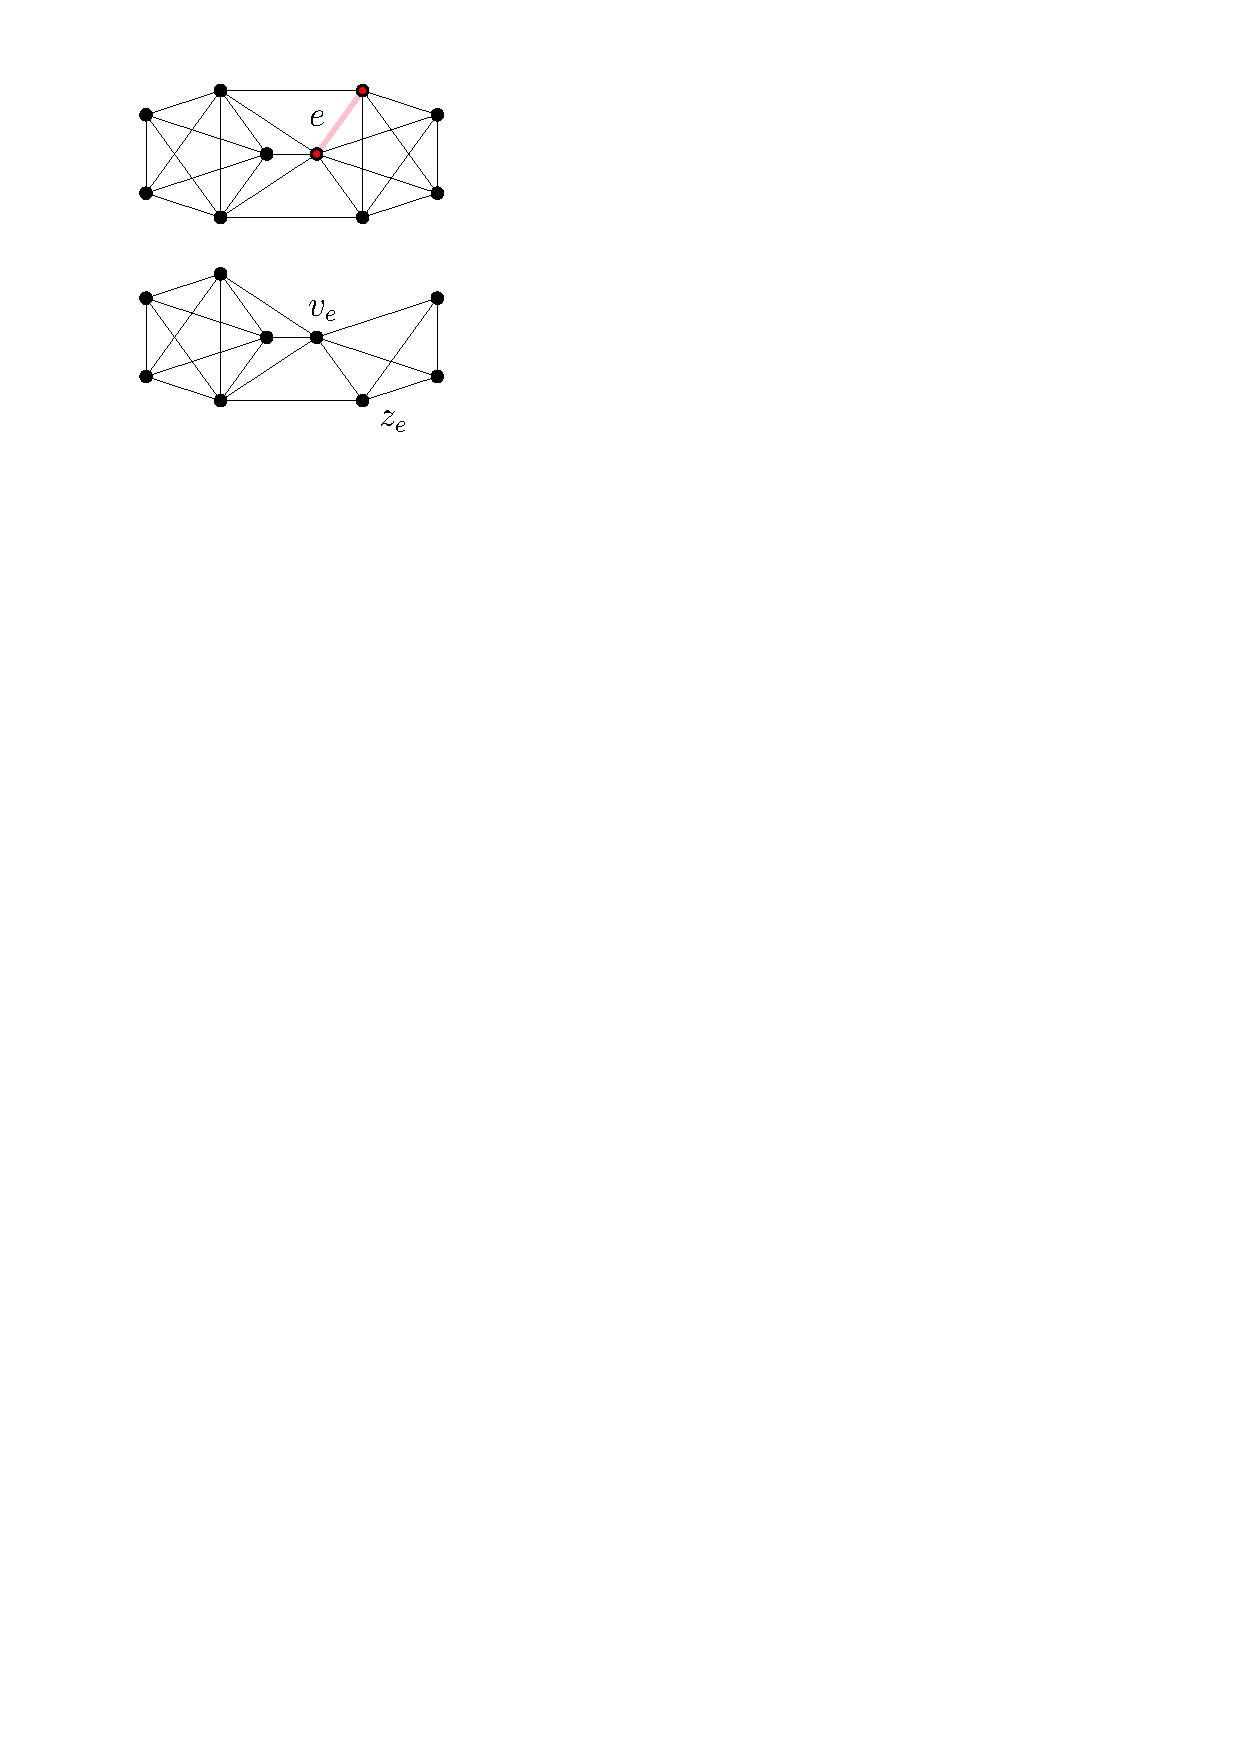
\includegraphics[width=0.14\textwidth]{figures/contractions_and_3_connectivity_01.pdf}
%\end{figure}


%\begin{figure}[ht]
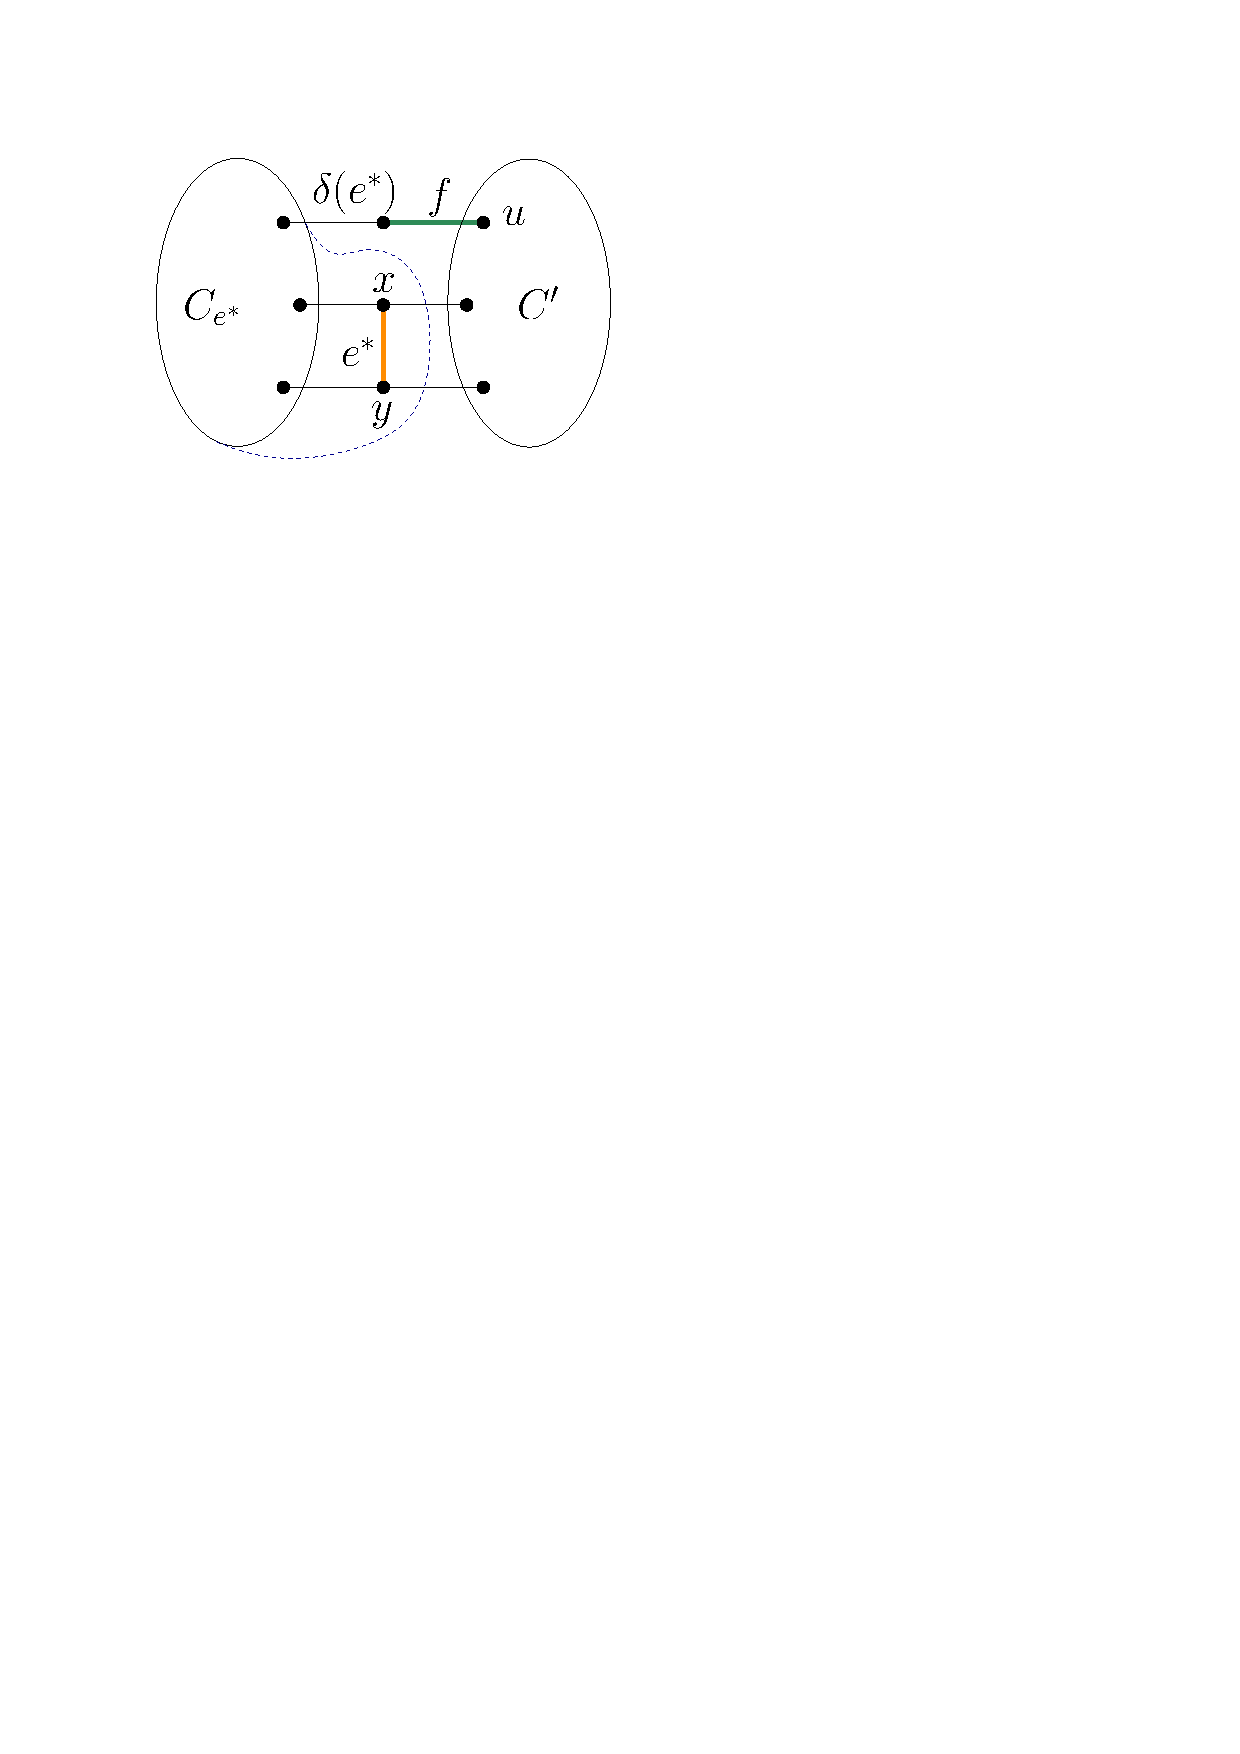
\includegraphics[width=0.24\textwidth]{figures/contractions_and_3_connectivity_03.pdf}
%\end{figure}
\end{paracol}



%%%%%%%%%%%%%%%%%%%%%%%%%%%%%%%%%%%%%%%%%%%%%%%%%%%%%%%%%%%%%%%%%%%%%%%%%% Tutte
\begin{lemma}\label{lemma:tutte}
$G = (V, E)$ が$3$-連結でクラトフスキー部分グラフを持たないなら、
$G$は平面埋込みを持つ。
\end{lemma}



\vspace*{-\intextsep}
\setcolumnwidth{0.82\textwidth, 0.18\textwidth}
\begin{paracol}{2}

\begin{proof}
頂点の個数に関する帰納法を用いる。
最小の$3$-連結グラフは$K_4$であり、
これは三頂点を適当に配置した後に残りの頂点を重心に配置することで平面埋め込みを得る。

$G = (V, E)$ に平面埋込みが存在することを示すために、
ある辺$e\in E$の縮約$G / e$が平面埋込みを持つと仮定する。
$v_e$ を$e=(x,y)$を縮約することで得られる$G / e$の頂点とする。
$G/e$は\cref{lemma:contractions_preserve_3_connectivity}より$3$-連結なので、
$v_e$ を除去すると多角形としての面$f$が出現する。

系列$(x_1, \ldots, x_k)$ を$x$に隣接する頂点で
$f$に沿った整列とする。
$y$ のすべての隣接頂点$y_1, \ldots, y_\ell$が$x_i$と$x_{i+1}$の間に配置されるなら、
$x$を$v_e$の位置に$y$を$x, y_1, \ldots, y_\ell$ の重心に配置することで
$G$ の平面埋込みを得る。
それ以外の二通りの場合はいずれも主張の前提に反する。
一つは、$x, y$が少なくとも3つの共通する隣接頂点を持つ場合で、
これは$G$が$K_5$の細分を持つ。
他方は、$x_i \neq y_1$および$x_{i+1} \neq y_\ell$の下で
$f$の境界上に
$x_i, y_1, \ldots, x_{i+1}, \cdots, y_\ell$の順で並んでいる場合で、
これは$G$が$K_{3,3}$の細分を持つ。
\end{proof}

%凸配置に関する言及はタットのばね定理に従う。

\switchcolumn
\vspace{0.5\intextsep}
\centering
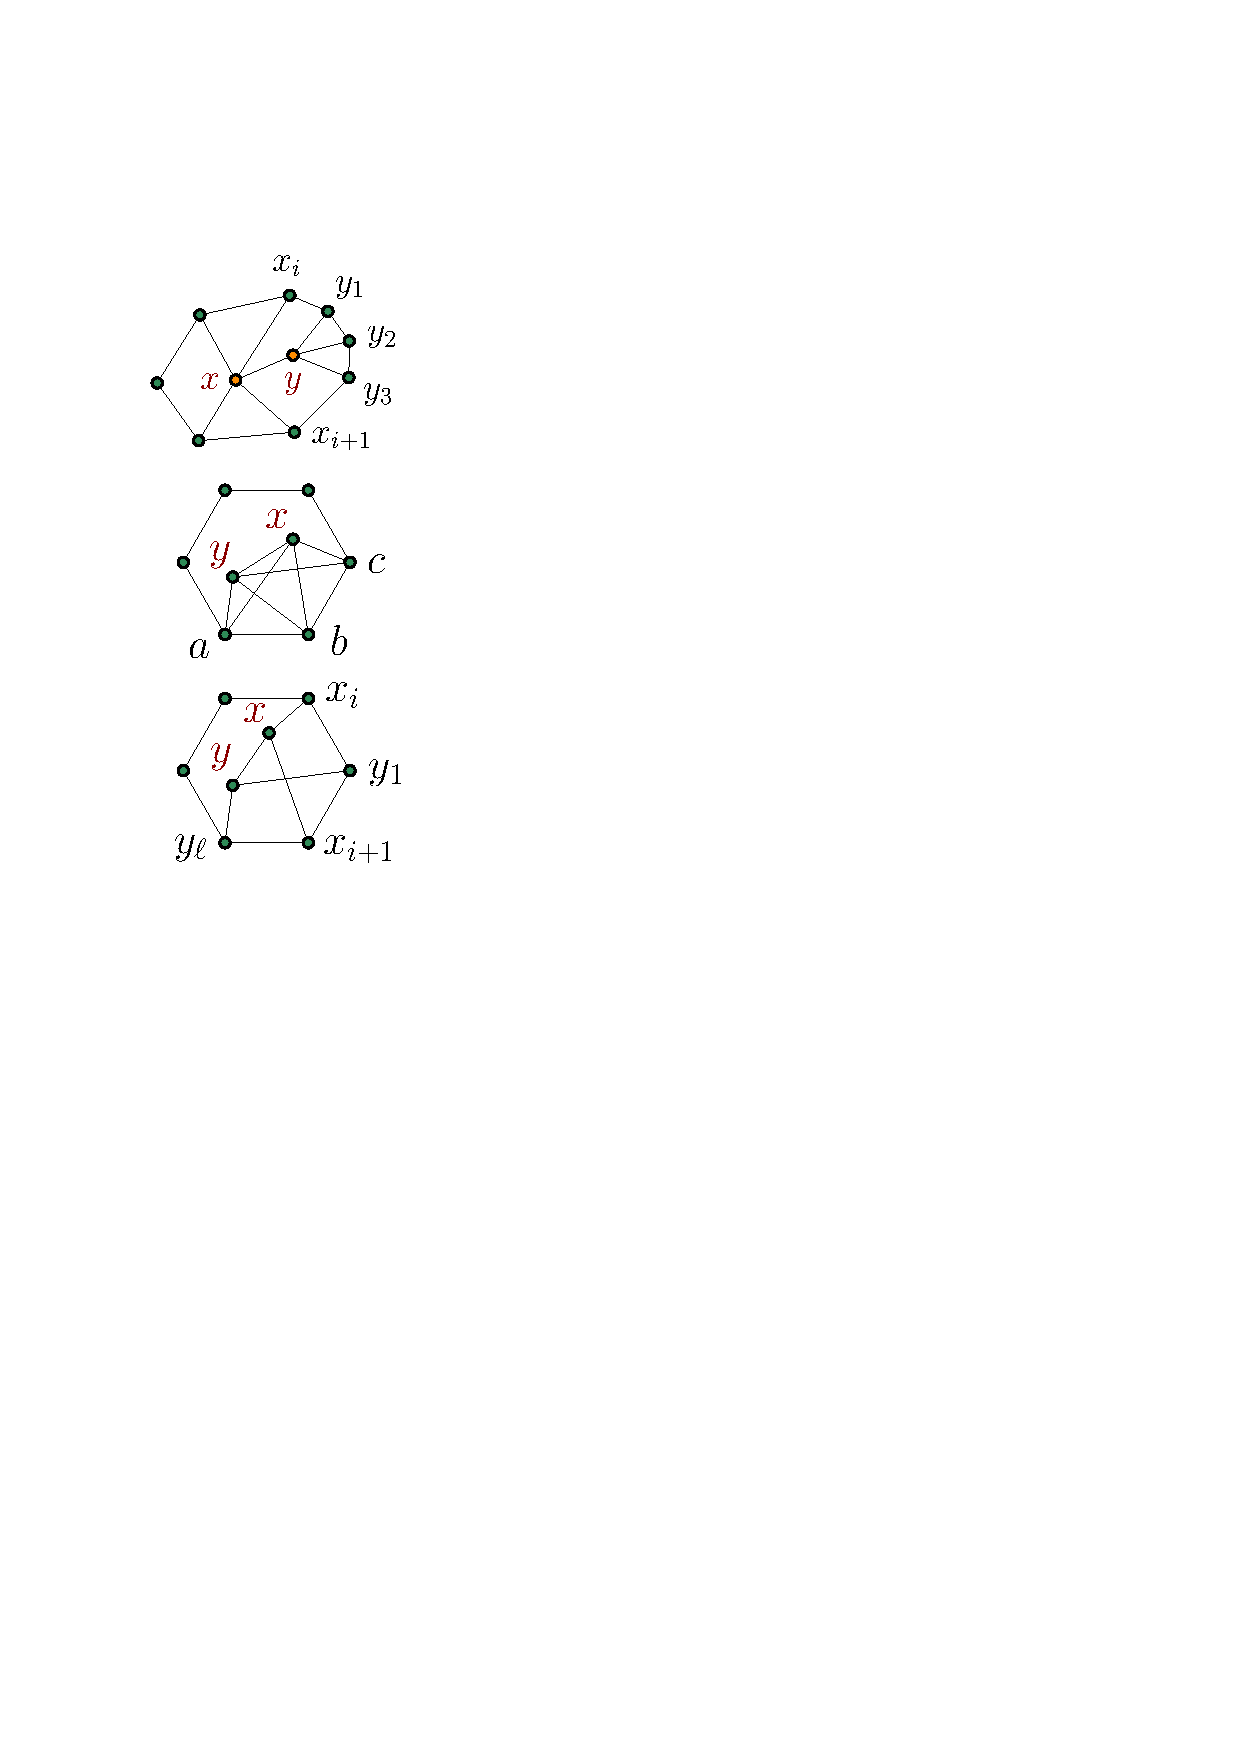
\includegraphics[width=0.12\textwidth]{figures/convex_embedding.pdf}
\end{paracol}

\begin{comment}
%\vspace*{-\intextsep}
\setcolumnwidth{0.85\textwidth, 0.15\textwidth}
\begin{paracol}{2}
\begin{theorem}[タットのばね定理]
単純で$3$-連結な平面的グラフは次の特徴を有する平面描画を持つ。各辺は直線分。
外面は凸多角形。内部の頂点は隣接頂点の重心。
\end{theorem}

\switchcolumn
\vspace*{-0.5\intextsep}
\begin{figure}[ht]
\centering
\includegraphics[width=0.12\textwidth]{figures/tutte_embedding_error.png}

{\small フルフトグラフの凸埋め込み}
\end{figure}

\end{paracol}

\end{comment}

